%%%%%%%%%%%%%%%%%%%%%%%%%%%%%%%%%%%%%%%%%
% Document Author: Plinio H. Vargas
% Course: CS-532, Spring 2016 at Old Dominion University
%
% Structured General Purpose Assignment
% LaTeX Template
%
% This template has been downloaded from:
% http://www.latextemplates.com
%
% Original template author:
% Ted Pavlic (http://www.tedpavlic.com)
%
% Note:
% The \lipsum[#] commands throughout this template generate dummy text
% to fill the template out. These commands should all be removed when 
% writing assignment content.
%
%%%%%%%%%%%%%%%%%%%%%%%%%%%%%%%%%%%%%%%%%
%----------------------------------------------------------------------------------------
%	PACKAGES AND OTHER DOCUMENT CONFIGURATIONS
%----------------------------------------------------------------------------------------

\documentclass{article}

\usepackage{fancyhdr} % Required for custom headers
\usepackage{lastpage} % Required to determine the last page for the footer
\usepackage{extramarks} % Required for headers and footers
\usepackage{listings}
\usepackage{graphicx} % Required to insert images
\usepackage{lipsum} % Used for inserting dummy 'Lorem ipsum' text into the template
\usepackage[bookmarks,bookmarksopen,bookmarksdepth=2]{hyperref} % for bookmarks
\usepackage{enumerate}
\usepackage{csquotes} % for quoting things
\usepackage{multirow}
\usepackage{amsmath}
\usepackage{caption}
\usepackage{navigator}%\usepackage{caption}
\usepackage[shortlabels]{enumitem}
\usepackage{enumitem}
\usepackage{lmodern}
\usepackage[utf8]{inputenc}
%\usepackage[table]{xcolor}% http://ctan.org/pkg/xcolo
\usepackage[dvipsnames]{xcolor}
\usepackage{longtable}
\usepackage{textcomp}
\usepackage{url}
\usepackage{import}
\usepackage{float}
\usepackage{dashrule} % for dashline
\usepackage{keystroke}
\usepackage{amssymb}
\usepackage{booktabs}

\lstdefinestyle{numbers}
{ frame=tb,
  language=python,
  aboveskip=3mm,
  belowskip=3mm,
  showstringspaces=false,
  columns=flexible,
  basicstyle={\small\ttfamily},
  numbers=left,
  numberstyle=\tiny\color{gray},
  keywordstyle=\color{blue},
  commentstyle=\color{OliveGreen},
  stringstyle=\color{purple},
  breaklines=true,
  breakatwhitespace=true,
  tabsize=3
}

\lstdefinestyle{nonumbers}
{ frame=shadowbox,
  language=python,
  aboveskip=3mm,
  belowskip=3mm,
  showstringspaces=false,
  columns=flexible,
  basicstyle={\small\ttfamily},
  numbers=none,
  numberstyle=\tiny\color{gray},
  keywordstyle=\color{blue},
  commentstyle=\color{OliveGreen},
  stringstyle=\color{purple},
  breaklines=true,
  breakatwhitespace=true,
  tabsize=3
}

\lstdefinestyle{mybox}
{
	basicstyle={\small\ttfamily},
    numbers=left,
    numberstyle=\tiny\color{gray},
    stepnumber=1,
    numbersep=5pt,
    showspaces=false, % don't show spaces by adding underscores
    showstringspaces=false, % don't underline spaces in strings
    showtabs=false, % don't show tabs with underscores
    frame=shadowbox,
    tabsize=4,
    captionpos=b,
    breaklines=true,
    breakatwhitespace=false,
  	keywordstyle=\color{blue},
	commentstyle=\color{OliveGreen},
  	stringstyle=\color{purple},    
    rulesepcolor=\color{red!20!green!20!blue!20},
    numberbychapter=false,
    stringstyle=\color{purple},
}


\providecommand{\providehyphenmins}[2]{}

% Margins
\topmargin=-0.45in
\evensidemargin=0in
\oddsidemargin=0in
\textwidth=6.5in
\textheight=9.0in
\headsep=0.25in 

\linespread{1.1} % Line spacing
\newcommand*{\mednu}{\mathbin{\scalebox{1.5}{$\nu$}}}% increase size of tau
\newcommand*{\medn}{\mathbin{\scalebox{1.1}{n}}}% increase size of letter a
\newcommand\multibrace[3]{\rdelim\}{#1}{3mm}[\pbox{#2}{#3}]}

% Set up the header and footer
\pagestyle{fancy}
\lhead{\hmwkAuthorName} % Top left header
\chead{\hmwkShortClass\ (\hmwkClassInstructor\ \hmwkClassTime): \hmwkShortTitle} % Top center header
%\rhead{\firstxmark} % Top right header
\rhead{} % Top right header
\lfoot{\lastxmark} % Bottom left footer
\cfoot{} % Bottom center footer
\rfoot{Page\ \thepage\ of\ \pageref{LastPage}} % Bottom right footer
\renewcommand\headrulewidth{0.4pt} % Size of the header rule
\renewcommand\footrulewidth{0.4pt} % Size of the footer rule

\setlength\parindent{0pt} % Removes all indentation from paragraphs

%----------------------------------------------------------------------------------------
%	DOCUMENT STRUCTURE COMMANDS
%	Skip this unless you know what you're doing
%----------------------------------------------------------------------------------------

% Header and footer for when a page split occurs within a problem environment
\newcommand{\enterProblemHeader}[1]{
\nobreak\extramarks{#1}{#1 continued on next page\ldots}\nobreak
\nobreak\extramarks{#1 (continued)}{#1 continued on next page\ldots}\nobreak
}

% Header and footer for when a page split occurs between problem environments
\newcommand{\exitProblemHeader}[1]{
\nobreak\extramarks{#1 (continued)}{#1 continued on next page\ldots}\nobreak
\nobreak\extramarks{#1}{}\nobreak
}

\newcounter{sub}[section]
\newenvironment{sub}[1][]{\stepcounter{sub}\thesub #1}{ }

\setcounter{secnumdepth}{4} % Removes default section numbers
\newcounter{homeworkProblemCounter} % Creates a counter to keep track of the number of problems
\newcommand{\sectionNumber}{\arabic{homeworkProblemCounter}.\sub }


\newcommand{\homeworkProblemName}{}
\newenvironment{homeworkProblem}[1][Problem \arabic{homeworkProblemCounter}]{ % Makes a new environment called homeworkProblem which takes 1 argument (custom name) but the default is "Problem #"
\stepcounter{homeworkProblemCounter} % Increase counter for number of problems
\setcounter{sub}{0}
\renewcommand{\homeworkProblemName}{#1} % Assign \homeworkProblemName the name of the problem
\
\section{\homeworkProblemName} % Make a section in the document with the custom problem count
\enterProblemHeader{\homeworkProblemName} % Header and footer within the environment
}{
\exitProblemHeader{\homeworkProblemName} % Header and footer after the environment
}

\newcommand{\problemAnswer}[1]{ % Defines the problem answer command with the content as the only argument
\noindent\framebox[\columnwidth][c]{\begin{minipage}{0.98\columnwidth}#1\end{minipage}} % Makes the box around the problem answer and puts the content inside
}

\newcommand{\homeworkSectionName}{}
\newenvironment{homeworkSection}[1]{ % New environment for sections within homework problems, takes 1 argument - the name of the section
\renewcommand{\homeworkSectionName}{#1} % Assign \homeworkSectionName to the name of the section from the environment argument
\subsection{\homeworkSectionName} % Make a subsection with the custom name of the subsection
\enterProblemHeader{\homeworkProblemName\ [\homeworkSectionName]} % Header and footer within the environment
}{
\enterProblemHeader{\homeworkProblemName} % Header and footer after the environment
}
   
%----------------------------------------------------------------------------------------
%	NAME AND CLASS SECTION
%----------------------------------------------------------------------------------------

\newcommand{\hmwkTitle}{\\Assignment\ \#4: \\Ex 8.3, 8.4, 9.4, 9.8 \& 9.10} % Assignment title
\newcommand{\hmwkShortTitle}{Assignment 4} % Assignment title
\newcommand{\hmwkDueDate}{Thursday,\ December 8,\ 2016} % Due date
\newcommand{\hmwkClass}{CS-734/834 Introduction to Information Retrieval} % Course/class
\newcommand{\hmwkShortClass}{CS-734/834 Intro to IR} % Course/class
\newcommand{\hmwkClassTime}{- Fall 2016} % Class/lecture time
\newcommand{\hmwkClassInstructor}{Dr.  Michael L. Nelson} % Teacher/lecturer
\newcommand{\hmwkAuthorName}{Plinio Vargas} % Your name
\newcommand{\hmwkAuthorEmail}{pvargas@cs.odu.edu} % Your name
%------------------------------------------------------------
% Algorithm declaration
%------------------------------------------------------------
\lstnewenvironment{algorithm}[1][] %defines the algorithm listing environment
{   
    %\refstepcounter{nalg} %increments algorithm number
    \captionsetup{labelsep=colon} %defines the caption setup for: it ises label format as the declared caption label above and makes label and caption text to be separated by a ':'
    \lstset{ %this is the stype
        frame=tB,
        numbers=left, 
        mathescape=true,
        numberstyle=\tiny,
        basicstyle={\small\ttfamily}, 
        keywordstyle=\color{blue}\bfseries\em,
        keywords={,input, output, return, 
                   datatype, function, in, 
                   if, else, for, foreach, 
                   while, write, begin, end, 
        } %add the keywords you want, or load a language as Rubens explains in his comment above.
        numbers=left,
        xleftmargin=.04\textwidth,
        #1 % this is to add specific settings to an usage of this environment (for instnce, the caption and referable label)
    }
}
{}
%----------------------------------------------------------------------------------------
%	TITLE PAGE
%----------------------------------------------------------------------------------------

\title{
\vspace{2in}
\textmd{\textbf{\hmwkClass:\ \hmwkTitle}}\\
\normalsize\vspace{0.1in}\small{Due\ on\ \hmwkDueDate}\\
\vspace{0.1in}\large{\textit{\hmwkClassInstructor\ }}
\vspace{3in}
}

\author{\textbf{\hmwkAuthorName} \\ \hmwkAuthorEmail}
\date{} % Insert date here if you want it to appear below your name

%----------------------------------------------------------------------------------------
%	EMBEDDED FILE
%----------------------------------------------------------------------------------------
%\embeddedfile{KarateClub}{../KarateClub.py}
%\embeddedfile{DrawOriginalClub}{../DrawOriginalClub.py}
%----------------------------------------------------------------------------------------
%	START OF DOCUMENT
%----------------------------------------------------------------------------------------
\begin{document}

\clearpage\maketitle
\thispagestyle{empty}

%----------------------------------------------------------------------------------------
%	TABLE OF CONTENTS
%----------------------------------------------------------------------------------------

%\setcounter{tocdepth}{1} % Uncomment this line if you don't want subsections listed in the ToC

\newpage
\clearpage\tableofcontents
\listoffigures
\lstlistoflistings
\listoftables

\thispagestyle{empty}
\newpage
\setcounter{page}{1}

%Exercices on pages: 35,52,
%----------------------------------------------------------------------------------------
%	Problem 1
%----------------------------------------------------------------------------------------
\begin{homeworkProblem}[Exercise 8.3]% Custom section title
\vspace*{10pt} % Question
For one query in the CACM collection (provided at the book website), generate
a ranking using Galago, and then calculate average precision, NDCG at 5
and 10, precision at 10, and the reciprocal rank by hand.

\subsection{Approach}
The CACM collection query log has a great deal of queries with a large number of words. This makes the query results in Galago somewhat difficult to interpret without some type of description of what should be considered as relevant result. For example, the TREC query log contains a narrative of what to consider in order to mark a document relevant. This is not the case for the CACM collection. Below, it is an example of the narrative found in the TREC collection.

\begin{verbatim}
<narr> Narrative: 
Relevant documents must include details of how pet! or animal!assisted 
therapy is or has been used.  Relevant details include information 
about pet therapy programs, descriptions of the circumstances in which 
pet therapy is used, the benefits of this type of therapy, the degree 
of success of this therapy, and any laws or regulations governing it.
\end{verbatim}

\vspace*{10pt} % Question
The $12^{th}$ query in the log was used for this exercise:

\begin{verbatim}
</DOC>
<DOC>
<DOCNO> 12 </DOCNO>
 portable operating systems
</DOC>
\end{verbatim}

\vspace*{10pt} % Question
A scale of 0 through 3 was used. Where 3 is the most relevant and 0 is not relevant. The following was the criteria used to determine the document's query result relevance:
\begin{itemize}
\item If the document is related to  ``portable operating system'', 3 points were awarded
\item If the document refers to “portable software”, 2 points were awarded
\item If the document is related to  “operating system”, at least 1 point was awarded
\item The occurrence of the word “portable” unrelated to operating system provided no relevance to the query
\end{itemize}

\subsection{Solution}
After placing ``portable operating system'' in \textbf{Galago}, the 10 first results were analyzed for relevance.

\begin{center}
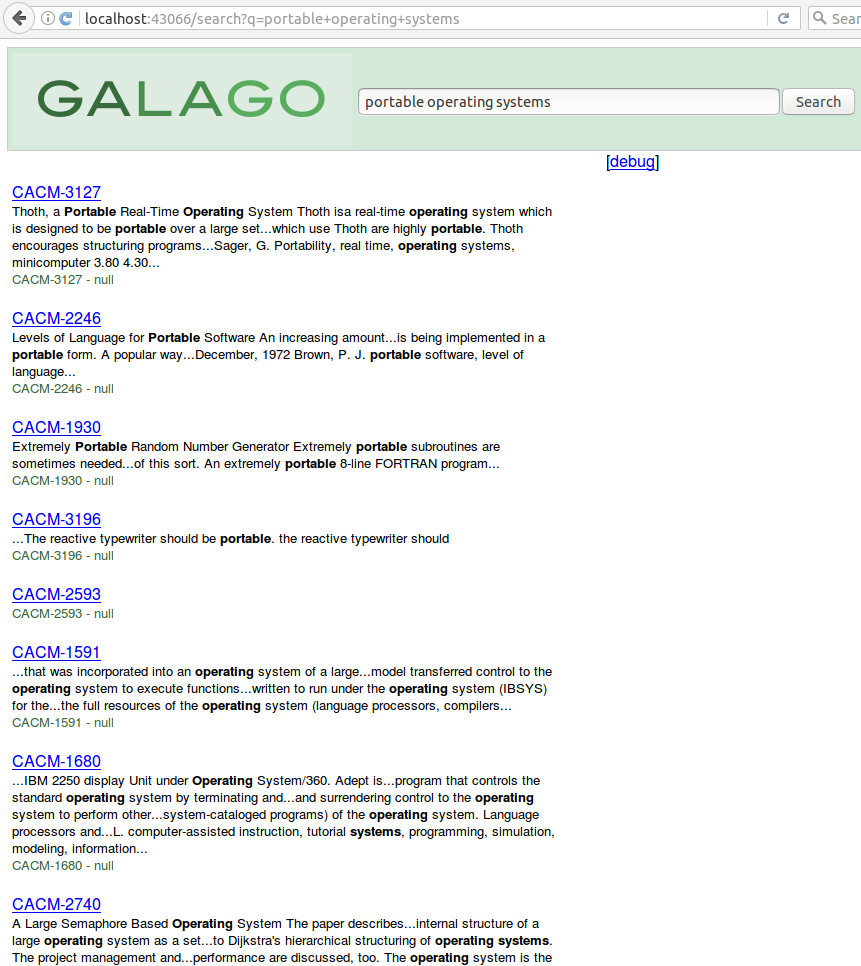
\includegraphics[scale=.5]{images/galago-search1.png}
\end{center}

\newpage
\subsubsection{Generated Ranking Using Galago}
Using the \textbf{relevance criteria} mentioned, the following scores were given to the ten retrieved documents:

\import{./}{table-1.tex}

\subsubsection{Calculating Recall and Precision}
\textbf{Recall Calculation}\\
By looking at Table \ref{tab:rank1}, the \textit{recall} calculation of the $i^{th}$  document $d$  resulting from \textbf{Query\#1} as follows:\\

\begin{equation}\label{eq:recall-cal}
	r_i =  \frac{\sum\limits_{k=1}^i d_k \Bigg  \{ d_k = 1\ if\ d_k\ is\ relevant\ 0\ otherwise }{|Query1|}
\end{equation}

$|Query1| = $total number of documents returned in Query\#1. \\
%
\vspace{5mm}\\
In other words, the \textit{recall} calculation $r_i$ of the $i^{th}$ ranked document $d$ that resulted from Query\#1 is equal to the count of relevant documents retrieved from the $1^{st}$ ranked to the $i^{th}$ ranked, divided by the total number of relevant documents related to the query.\\
%
\vspace{5mm}\\
\textbf{Precision Calculation}\\
By looking at Table \ref{tab:rank1}, the \textit{precision} calculation of the $i^{th}$  document $d$  resulting from \textbf{Query\#1} as follows:\\

\begin{equation}\label{eq:precision-cal}
	p_i =  \frac{\sum\limits_{k=1}^i d_k \Bigg  \{ d_k = 1\ if\ d_k\ is\ relevant\ 0\ otherwise }{i}
\end{equation}
\vspace{5mm}\\
In other words, the \textit{precision} calculation $p_i$ of the $i^{th}$ ranked document $d$ that resulted from Query\#1 is equal to the count of relevant documents retrieved from the $1^{st}$ ranked to the $i^{th}$ ranked, divided by the rank of the  $i^{th}$ document related to the query.\\

By applying equations (\ref{eq:recall-cal}) and (\ref{eq:precision-cal}) to the values of Table \ref{tab:rank1}, it resulted in the \textit{recall} and \textit{precision} calculation shown on Table \ref{tab:rank1cal}.\\

\textbf{Summary}\\
\begin{center}
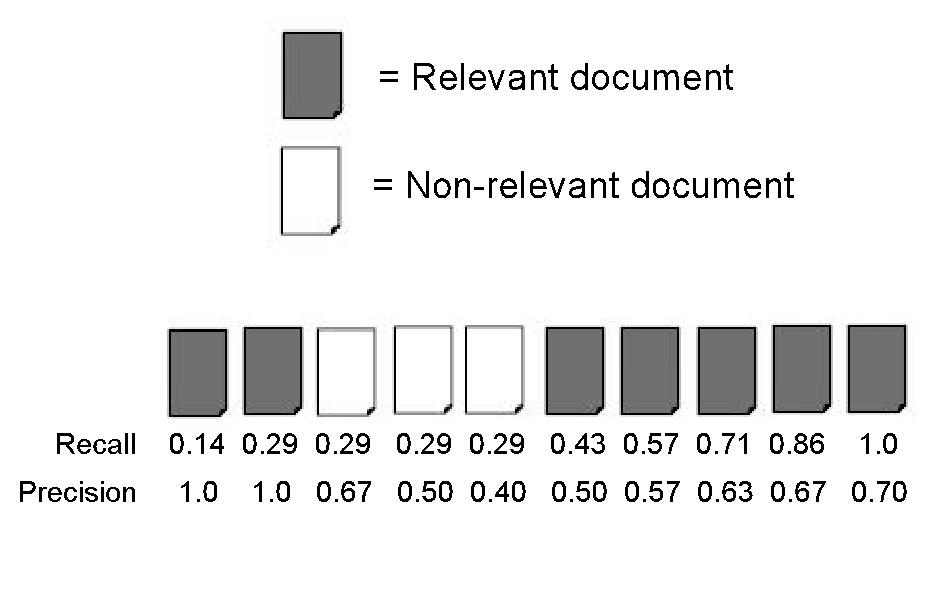
\includegraphics[scale=.5]{images/result1.pdf}
\end{center}

\import{./}{table-2.tex}

\subsubsection{Average Precision at 10}
From Table \ref{tab:rank1cal}, the Average Precision for Query \#1 (APQ1) is:
\begin{equation*}
	APQ1 = (1.0 + 1.0 + 0.57 + 0.63 + 0.67 + 0.70) / 6
\end{equation*}
\begin{equation*}
	APQ1 = 0.72
\end{equation*}

\newpage
\subsubsection{NDCG at 5}

\import{./}{table-3.tex}

\import{./}{table-4.tex}

Looking at Table \ref{tab:ndcg-at5-cal}:\\

NDCG at 5 = 0.74

\newpage
\subsubsection{NDCG at 10}

\import{./}{table-5.tex}

\import{./}{table-6.tex}

Looking at Table \ref{tab:ndcg-at10-cal}:\\

NDCG at 10 = 0.71

\subsubsection{Reciprocal Ranking}
According to \cite{CroftMetzlerStrohman}  \textit{reciprocal rank} ``is defined as the reciprocal of the rank at which the first relevant document is retrieved''. The first document of the query result is a relevant document. Then, the relevant ranking \textit{RR} can be determined by:
\begin{equation*}
RR = 1/1 = 1
\end{equation*}

\end{homeworkProblem}

%----------------------------------------------------------------------------------------
%	Problem 2
%----------------------------------------------------------------------------------------
\newpage
\begin{homeworkProblem}[Exercise 8.4]% Custom section title
\vspace*{10pt} % Question
For two queries in the CACM collection, generate two uninterpolated recall-precision graphs, a table of interpolated precision values at standard recall levels, and the average interpolated recall-precision graph.

\subsection{Approach}
In addition to query \#1, used on the previous exercise, the second query is shown below:
\begin{verbatim}
<DOC>
<DOCNO> 2 </DOCNO>
I am interested in articles written either by Prieve or Udo Pooch
Prieve, B.
Pooch, U.
</DOC>
\end{verbatim} 

\vspace*{10pt} % Question
A scale of 0 through 3 was used. Where 3 is the most relevant and 0 is not relevant. The following was the criteria used to determine the document's query result relevance:
\begin{itemize}
\item If any authors created the document, 3 points was awarded
\item If any of the authors appeared in the body of the document, 2 points were awarded
\item If the document was related to any of the writing of the authors, 1 point was  awarded
\item Any other condition 0 was awarded
\end{itemize}

\newpage
\subsection{Solution}
After placing query \#2 in \textbf{Galago}, the 10 first results were analyzed for relevance.

\begin{center}
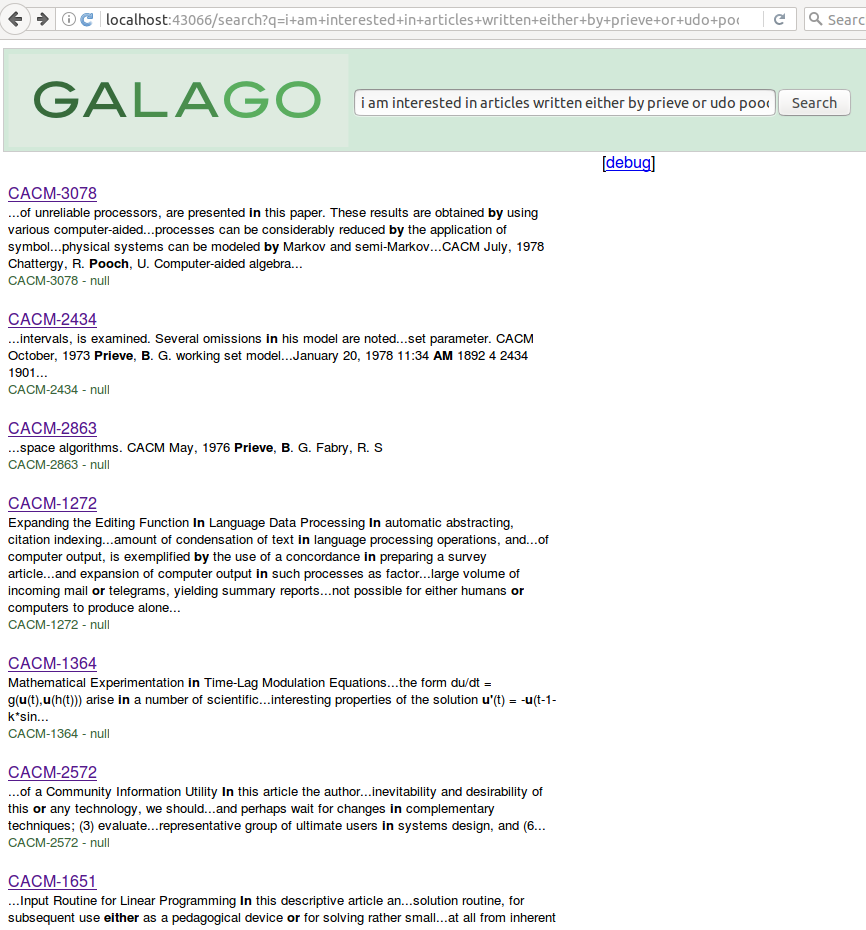
\includegraphics[scale=.5]{images/galago-search2.png}
\end{center}

The NDCG at 10 calculation for Query \#2 generated the following results:\\

\newpage
%\import{./}{table-7.tex}
%
%\import{./}{table-8.tex}
%
\newpage
\import{./}{table-9.tex}

\subsubsection{Uninterpolated Recall Precision Graph}
The \textbf{R} script \textit{query.R} was used to generate the graph.  The data for this graph can be seen on Table \ref{tab:precision-recall}.

\begin{center}
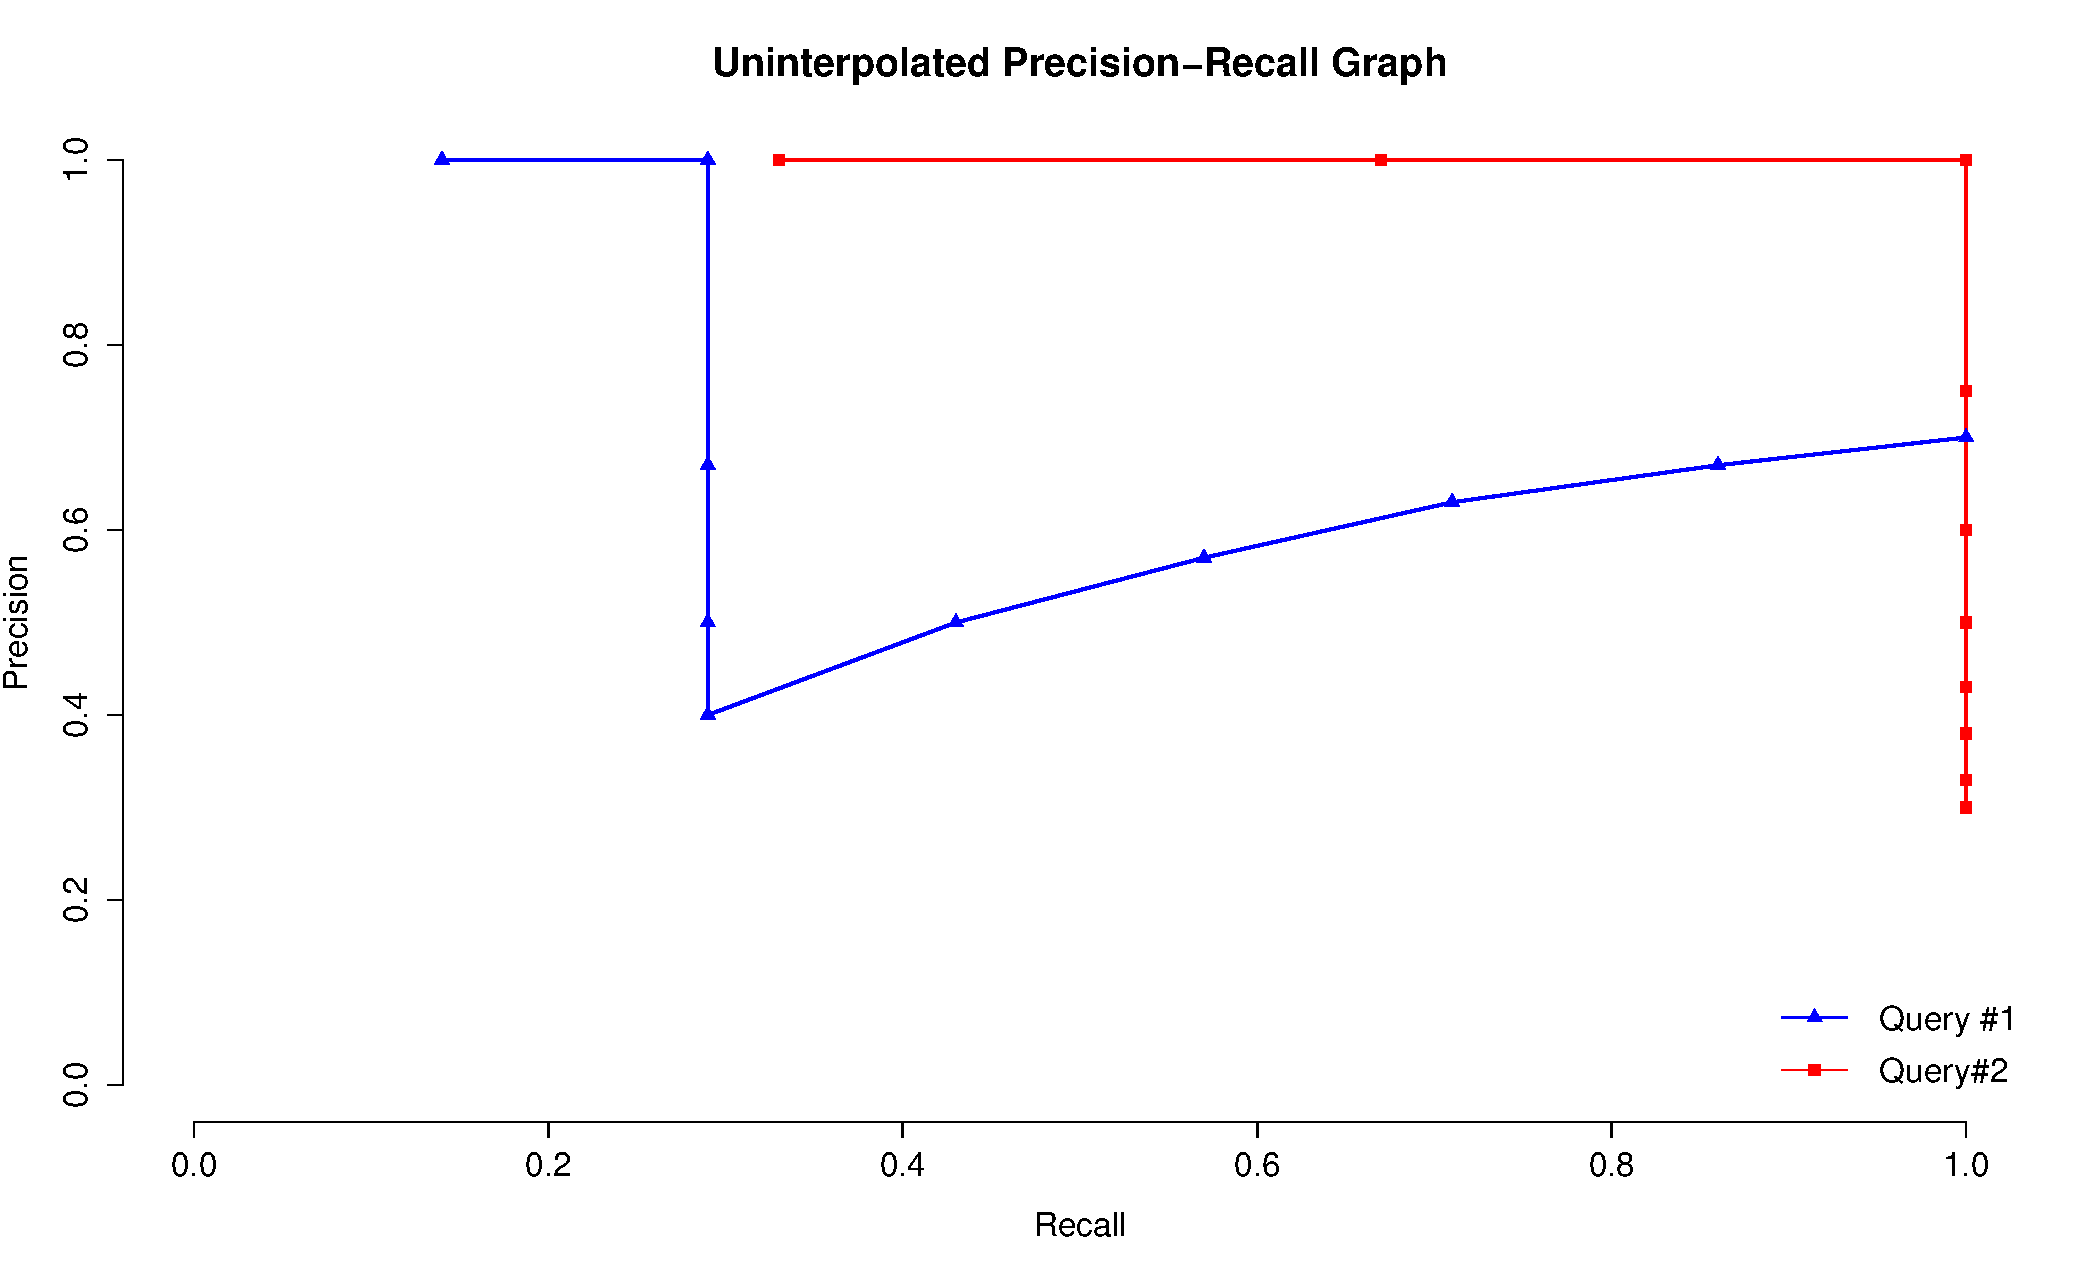
\includegraphics[scale=.5]{images/query.pdf}
\end{center}

\newpage
\subsubsection{Table of Interpolated Precision Values}
\import{./}{table-10.tex}

\subsubsection{Average Interpolated Recall-Precision Graph}
The \textbf{R} script \textit{avg-precision.R} was used to generate the graph.  The data for this graph can be seen on Table \ref{tab:precision-recall}.

\begin{center}
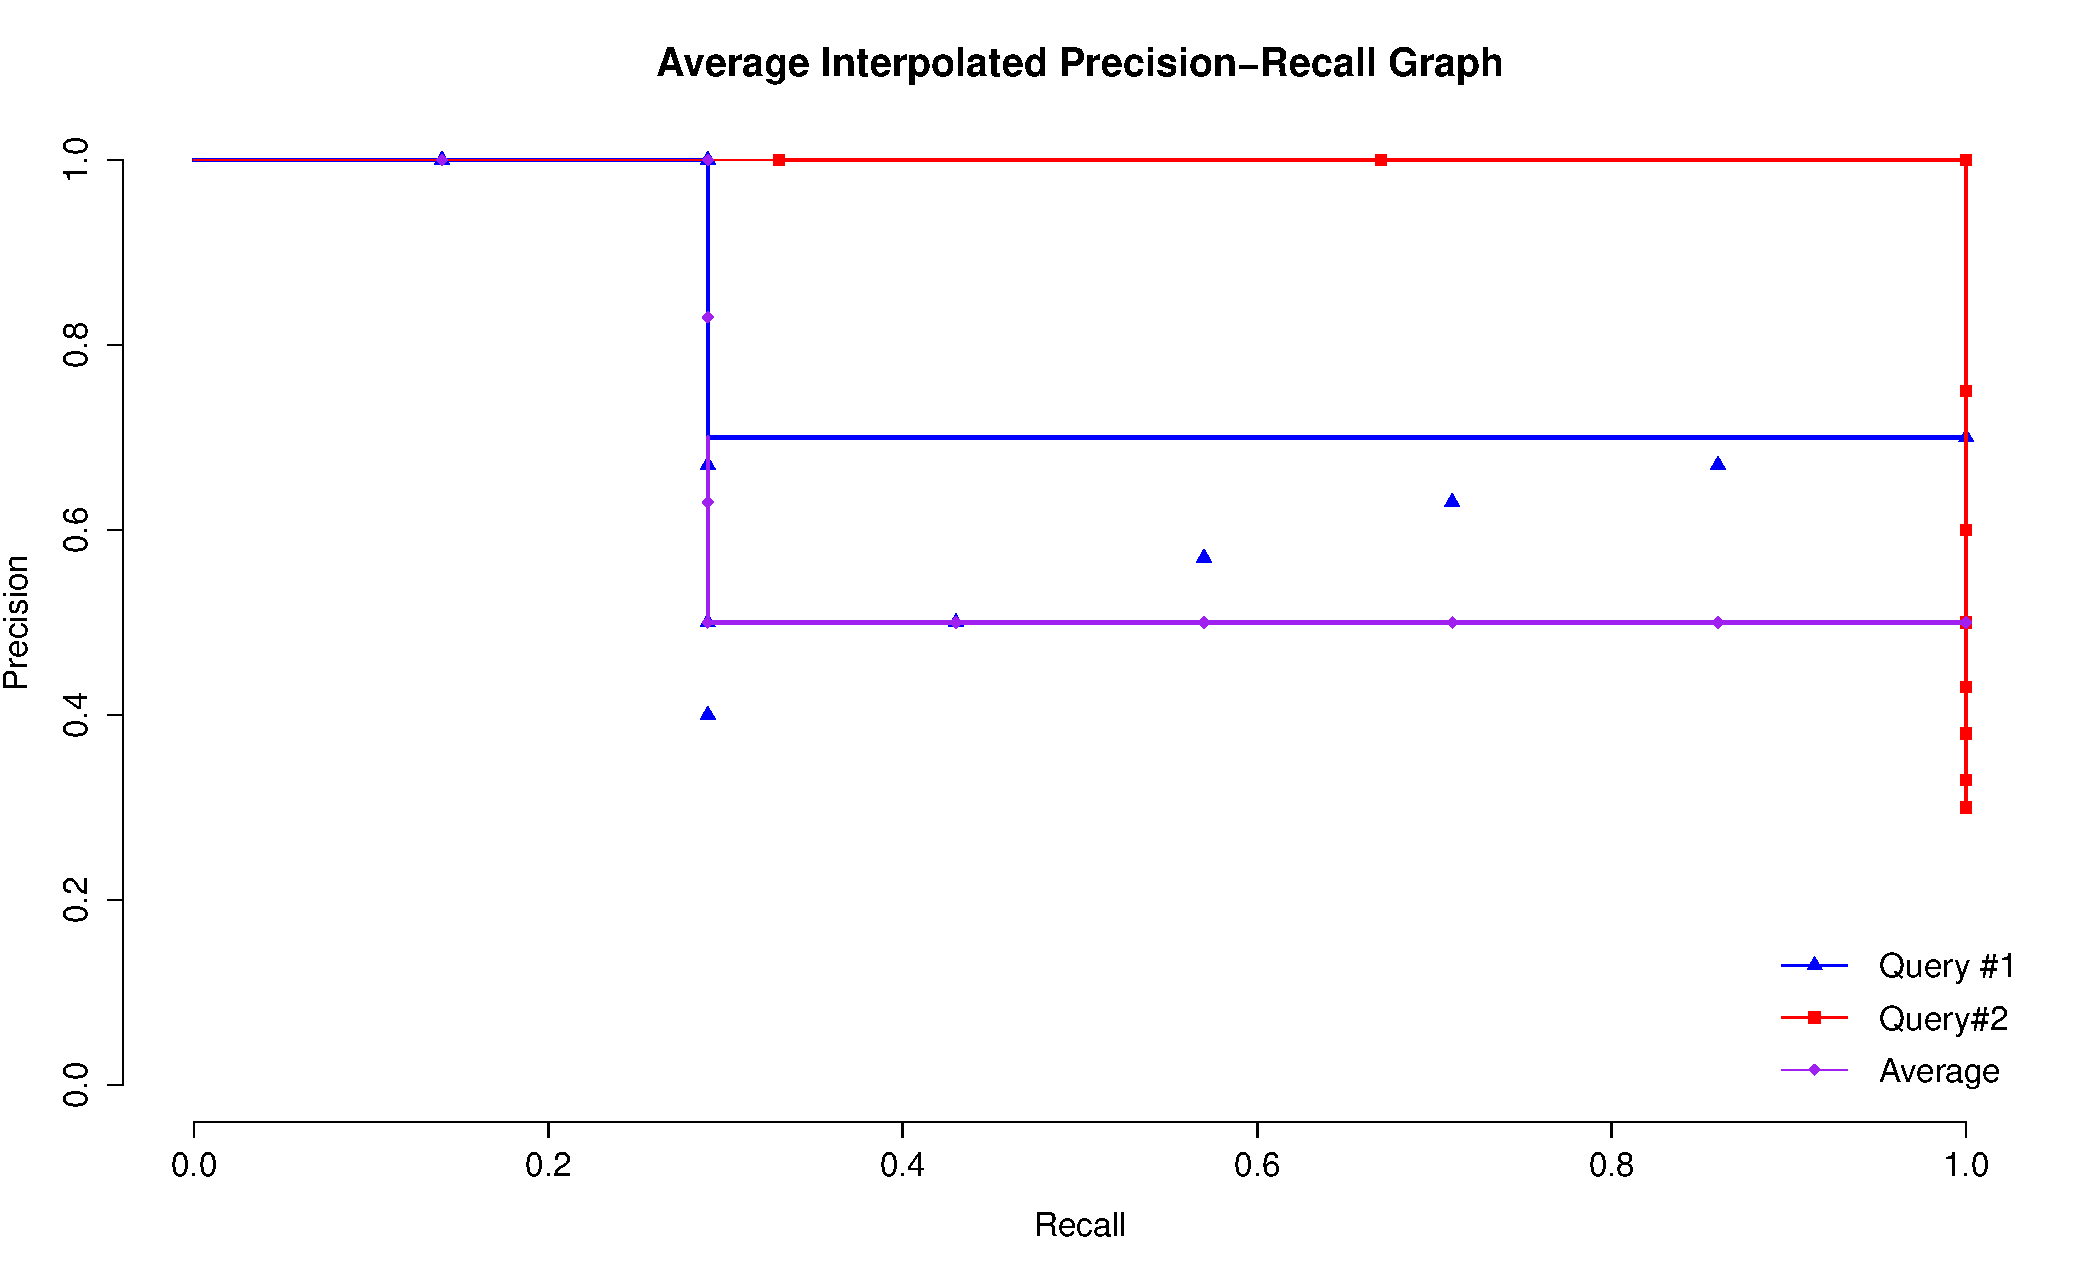
\includegraphics[scale=.5]{images/avg-recall-precision.pdf}
\end{center}

\end{homeworkProblem}

%----------------------------------------------------------------------------------------
%	Problem 3
%----------------------------------------------------------------------------------------
\newpage
\begin{homeworkProblem}[Exercise 9.4]% Custom section title
\vspace*{10pt} % Question
For some classification data set, compute estimates for $P(w|c)$ for all words
$w$ using both the multiple-Bernoulli and multinomial models. Compare the multiple-Bernoulli estimates with the multinomial estimates. How do they differ? Do the estimates diverge more for certain types of terms?

\subsection{Approach}
The CACM collection was used to obtain the data set. No stopwords were used. In order to eliminate the stopwords, the application from assignment \#2, \textit{zipf\_curve.py}, was used to determine the words containing the higher frequency. The next 20 highest frequency terms were selected, without including any numbers or non-relevant words which may be part of the index. 

\subsubsection{Data set Classification}
Considering that the CACM collection is related to computer science, the classification selection for this exercise were: \textbf{hardware} and \textbf{software}.\\

\subsubsection{Word List}
Table \ref{tab:word-sel} contains the list of the words used for this exercise. 
An evaluation was made using \textbf{Galago} to determine 20 documents relevant to \textbf{hardware} as the set to classify the term appearance probability for which our word list is present. A similar approach was used to obtain 20 documents relevant to the classification for \textbf{software}.

\import{./}{table-11.tex}

\newpage
\subsubsection{Document Classification Criteria}
Snippet information was used to consider if it was worthy to inspect the document for classification selection. If a document appeared to be related to software and hardware, it was discarded in order to have a good representation of the classified document.

\subsubsection{Generating the Data}
The \textbf{Python} script \textit{bernoulli-estimate.py} was developed to generate the data contained on Tables \ref{tab:bernoulli-estimate} and \ref{tab:multinomial-estimate}. The script read two files: \textit{hardware.txt} and \textit{software.txt}. Those files contain the documents in the collection considered related to a \textbf{hardware} and \textbf{software} query respectively for the training.  A dictionary variable \textit{word\_matrix} was passed as a parameter (line 178 of Listing \ref{listing:count-freq}) where the feature frequency is going to be stored. \\

If a training document corresponded to a \textit{hardware} classification, then a column with a value of 'H' was added to the row.  This action was the only step needed for training the document instance as \textit{hardware}. The same was done for the \textit{software} training document classification. See lines 215-218

%--------------
%  count terms
%--------------
\lstinputlisting[language=Python,
                 style=mybox, 
                 captionpos=t,
                 caption={Frequency of Term Count},
				 linerange={178-223},
				 firstnumber=178,                  
                 label=listing:count-freq,
                 ]
{../bernoulli-estimate.py}
%
\vspace{5mm}
Two functions were created to make the distinction while considering the presence of a term, used in the \textbf{multiple-bernoulli} method, or the frequency of the term, used in the \textit{multinomial} method. Looking at lines 152 through 155 on Listing \ref{listing:bernoulli-fucntion}, we can notice the function removed the frequency and converted any value greater than zero equal to 1. The \textbf{multinomial} function accomplished the same job, but it considered the frequency of the term instead of only its presence. 
%--------------
%  multiple-bernoulli
%--------------
\lstinputlisting[language=Python,
                 style=mybox, 
                 captionpos=t,
                 caption={Multiple-Bernoulli Function},
				 linerange={139-157},
				 firstnumber=139,                  
                 label=listing:bernoulli-fucntion,
                 ]
{../bernoulli-estimate.py}
%
\vspace{5mm}

\begin{center}
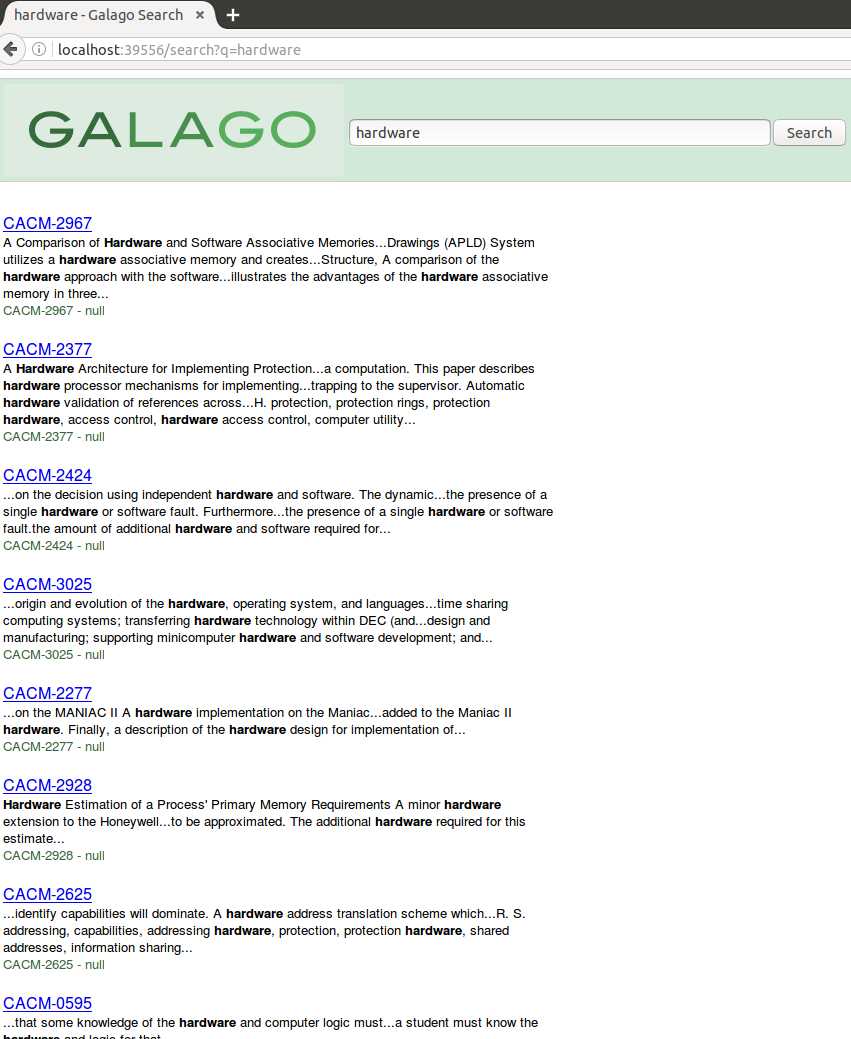
\includegraphics[scale=.5]{images/hardware-search.png}
\end{center}

\begin{center}
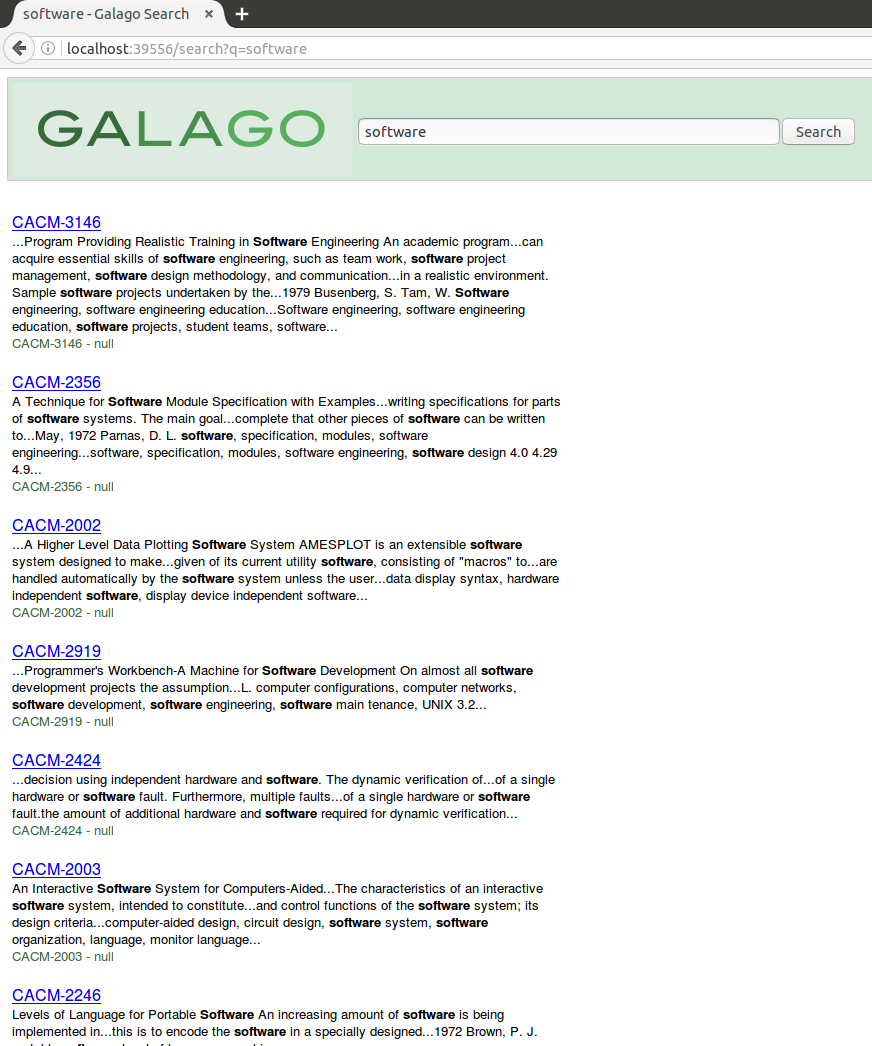
\includegraphics[scale=.5]{images/software-search.png}
\end{center}

\subsubsection{Multiple-Bernoulli Model}
$P(w|c)$ for all words on Table \ref{tab:word-sel}, using \textbf{multiple-Bernoulli} model, was calculated by applying the formula:

\begin{equation}
P(w|c) = \frac{df_{w,c} + 1}{N_c + 1}
\end{equation}

Where $df_{w,c}$ refers to the number of training documents with class label $c$ in which term $w$ occurs, and $N_c$ is the total number of training documents with class label $c$. Knowing that 20 training documents were used for each of the classifications in this exercise:
\begin{equation*}
N_{hardware} = 20
\end{equation*}
and,
\begin{equation*}
N_{software} = 20
\end{equation*}

\subsubsection{Multinomial Model}
$P(w|c)$ for all words on Table \ref{tab:word-sel}, using \textbf{multinomial} model, was calculated by applying the formula:

\begin{equation} \label{eq:muiltinomial}
P(w|c) = \frac{tf_{w,c} + 1}{|c| + |\mednu|}
\end{equation}

Where $tf_{w,c}$ refers to the number of times that term $w$ occurs in document $d$, $|c|$ is the total number of terms that occur in training documents with class label $c$. $|\mednu|$ is the number of features (20 words in our case) considered to classify the document. After scanning the collection for the selected training document, the following $|c|$ values resulted to provide input for equation (\ref{eq:muiltinomial}):

\begin{equation*}
|c_{hardware}| = 190
\end{equation*}
and,
\begin{equation*}
|c_{software}| = 137
\end{equation*}

\newpage
\subsection{Solution}

\subsubsection{Multiple-Bernoulli Model}
\import{./}{table-12.tex}

\newpage
\subsubsection{Multinomial Model}
\import{./}{table-13.tex}

\subsubsection{Multiple-Bernoulli vs Multinomial Estimates Comparison}
Table \ref{tab:bernoulli-estimate} and Table \ref{tab:multinomial-estimate} yielded the data to plot on Fig \ref{fig:probability-estimate}, the probability estimates for the \textit{Multiple-Bernoulli} and \textit{Mutinomial} models. As equation(\ref{eq:muiltinomial}) suggests, the probability estimates in the \textit{Multinomial} model are going to generate a much smaller value since in comparison with the \textit{Bernoulli} model, the denominator in equation (\ref{eq:muiltinomial}) is greater than in equation (\ref{fig:probability-estimate}).\\
Although, we are not trying to calculate the \textit{information gain} of the features for this data set, the graph can give us some information which can provide us with some insight. For example, there are various points on the graph in which pairs intercept.  In other words, both variables have the same probability estimate. The result for the \textit{Bernoulli} estimate (red and orange curves) shows that variables $\{7, 9, 10, 11, 16, 19\}$ have the same values. The values of those features are: \{system, problem, number, processing, languages, matrix\} respectively. \\
On the other hand, the \textit{Multinomial} model result does not have a single value in which the probability estimate is exactly the same. There are some instances where the probability appears to converge, but there is  still a very small percentage where a distinction could be made. According to the textbook \cite{CroftMetzlerStrohman}: ``in practice, the multinomial model has been shown to consistently outperform the multiple-Bernoulli model'', perhaps the reason for that is that we can make use of more features in the \textit{multinomial} model. In contrast, in the \textit{multiple-Bernoulli} model where the quantity of variable with equal estimate makes it more difficult to provide an accurate document classification.\\
However, about the same number of features (in our case the vairables $\{1, 9, 14, 19, 20\}$) in the \textit{multinomial} model has an estimate delta close to zero. A common denominator in these two sets are $\{9, 19\}$ (problem and languages). It makes prefect sense that these two words do not appear to add more information to distinguish or classify if a document is related to \textbf{hardware} or \textbf{software}. Looking at Table \ref{tab:bernoulli-estimate}, the word \textit{matrix} does not appear in any of the searched documents, and \textit{problem} is such a generic word that it probably could be used in any topic of the ACMC collection.\\

The \textbf{R} script used to create Fig \ref{fig:probability-estimate} was \textit{probability.R}
\begin{figure}
\caption{Probability Estimate}
\label{fig:probability-estimate}
\begin{center}
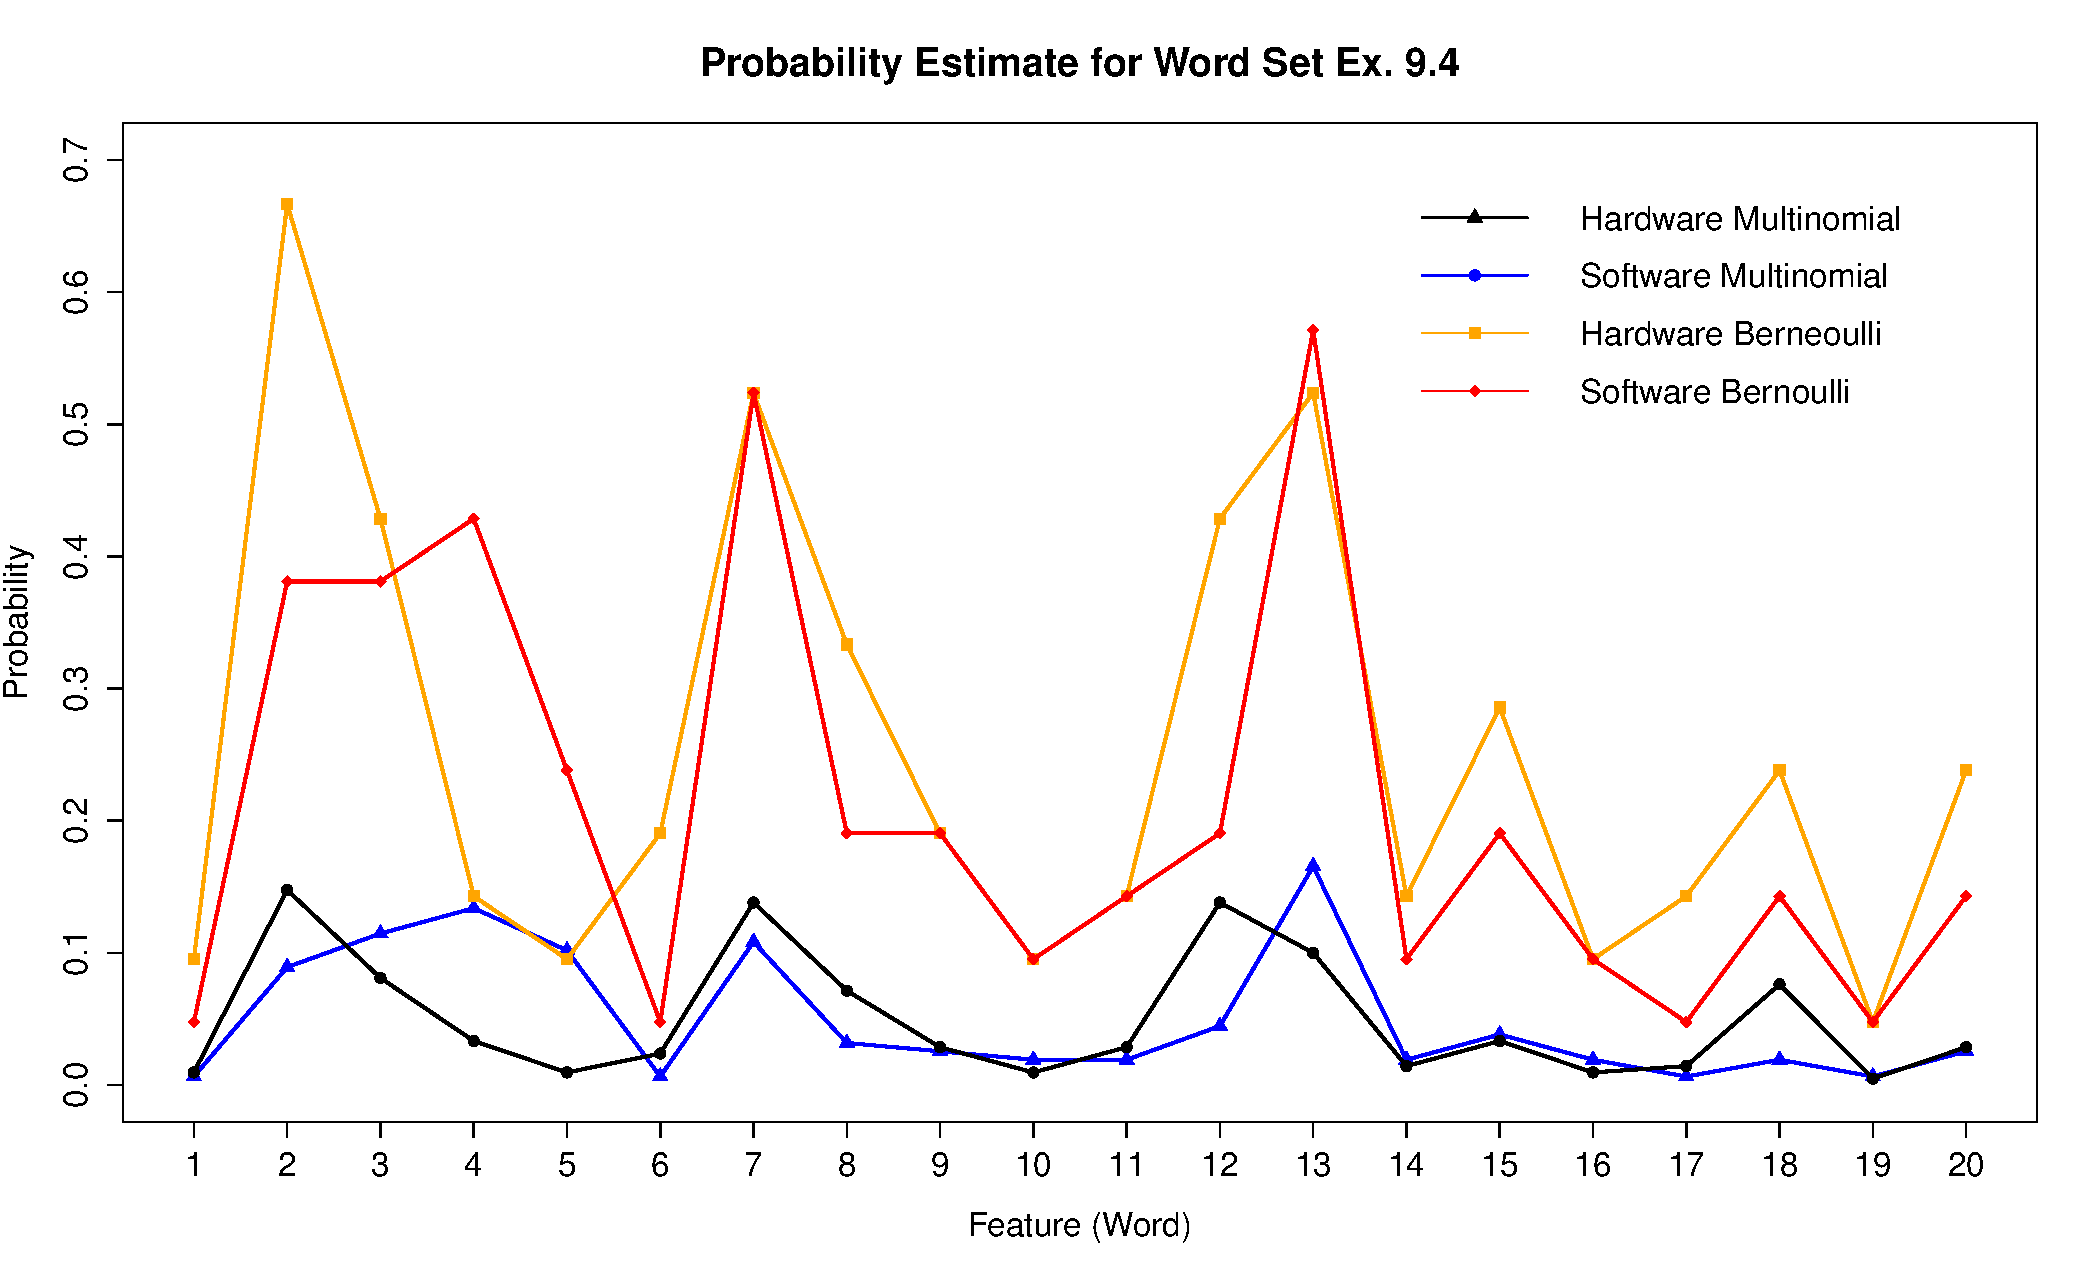
\includegraphics[scale=.5]{images/bernoulli-estimate.pdf}
\end{center}
\end{figure}
\end{homeworkProblem}

%----------------------------------------------------------------------------------------
%	Problem 4
%----------------------------------------------------------------------------------------
\newpage
\begin{homeworkProblem}[Exercise 9.8]% Custom section title
\vspace*{10pt} % Question
Cluster the following set of two-dimensional instances into three clusters using
each of the five agglomerative clustering methods:\\
(–4, –2), (–3, –2), (–2, –2), (–1, –2), (1, –1), (1, 1), (2, 3), (3, 2), (3, 4), (4, 3)\\
Discuss the differences in the clusters across methods. Which methods produce
the same clusters? How do these clusters compare to how you would manually
cluster the points?


\subsection{Approach}
\textbf{R} includes the package \textit{cluster} which contains a solution to the five agglomerative cluster methods: \textit{Single linkage}, \textit{Complete linkage}, \textit{Average linkage}, \textit{Average group linkage} and \textit{Ward’s method}. The name of the script that plotted the cluster is \textit{agnes.R}. The package has a function (\textit{agnes}) that produces a dendrogram of the clustered points.\\

In order to know how to group the dendrogram in \textit{k} number of clusters, \textbf{R} provides the function \textit{cutree} which divides the graph into \textit{k} partitions. A portion of the \textbf{R} scripts that performs this function is shown below:

\begin{verbatim}
groups <- cutree(ag, k=5) # cut tree into 3 clusters
rect.hclust(H.fit, k=5, border="red") 
\end{verbatim}

\subsection{Solution}
\subsubsection{Manual Clustering of Points}
Fig \ref{fig:personal} shows in highlighted green the way I would cluster the points with $k=3$. This is the same result shown for the five agglomerative methods.

\begin{figure}[h]
\caption{Manual Point Clustering with K=3}
\label{fig:personal}
\begin{center}
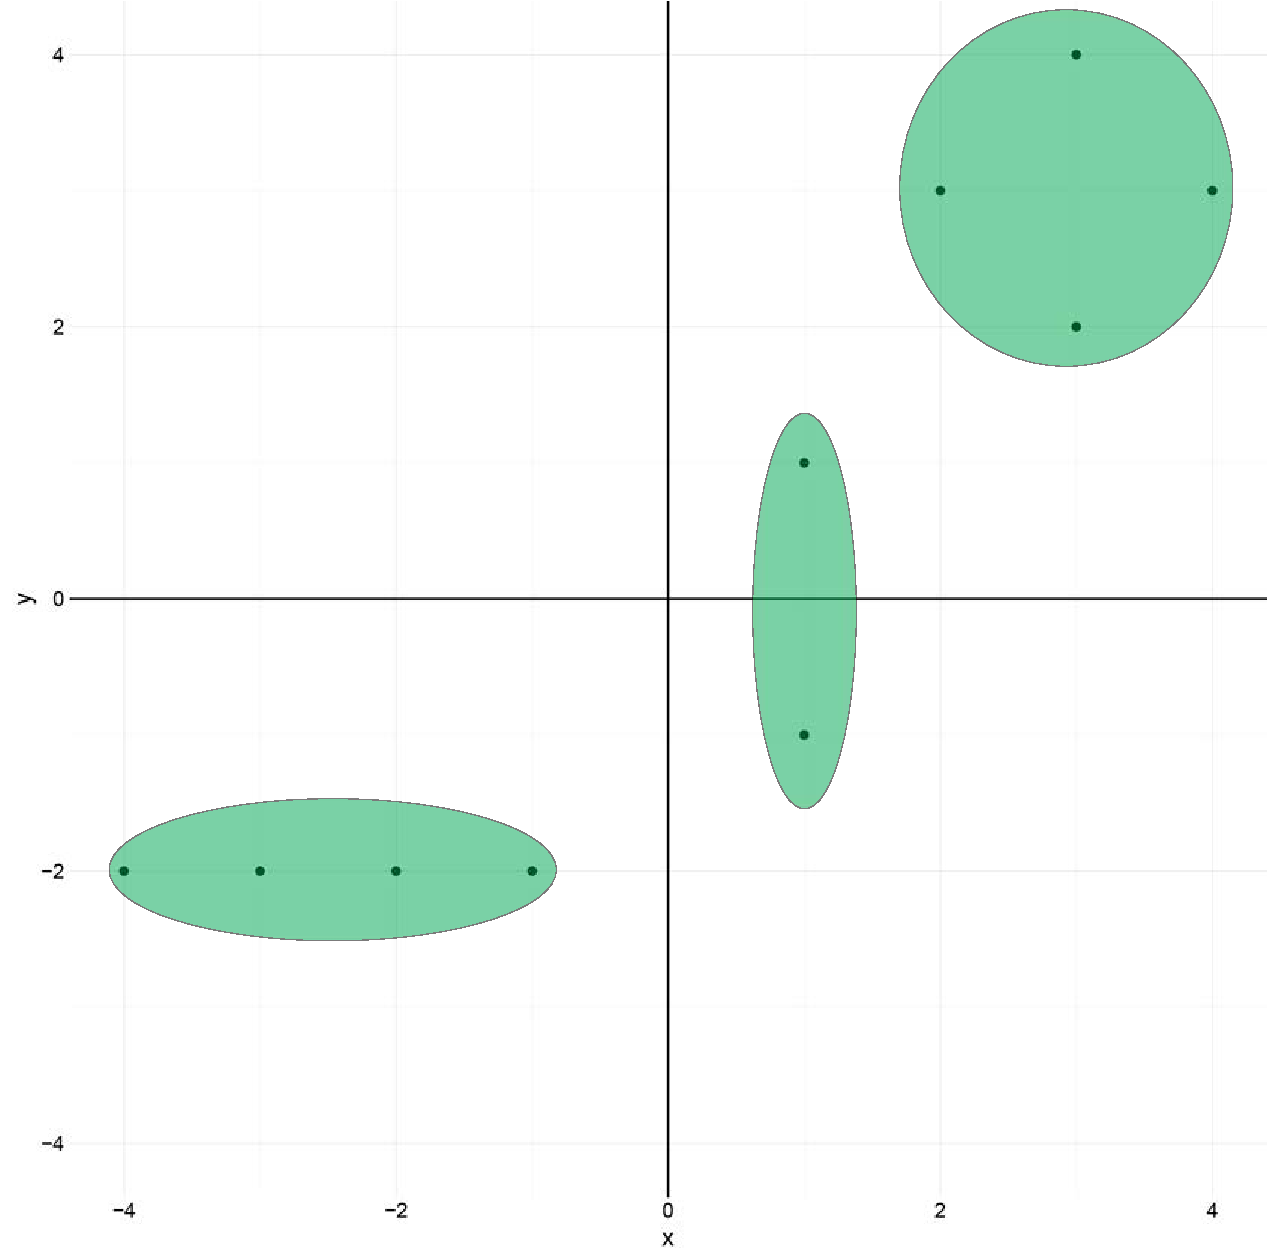
\includegraphics[scale=.30]{images/manual-cluster.pdf}
\end{center}
\end{figure}

\subsubsection{Single Linkage Method}
For this method \textbf{R} produced the following result:
\begin{verbatim}
Call:	 agnes(x = d, metric = "euclidean", method = "single") 
Agglomerative coefficient:  0.3892469 
Order of objects:
 [1]  1  2  3  4  5  6  7  8  9 10
Height (summary):
   Min. 1st Qu.  Median    Mean 3rd Qu.    Max. 
  1.000   1.000   1.414   1.524   2.000   2.236 

Available components:
[1] "order"  "height" "ac"     "merge"  "diss"   "call"   "method"
[8] "data" 
\end{verbatim}

\begin{figure}
\caption{Single Linkage Graph K=3}
\label{fig:singel}
\begin{center}
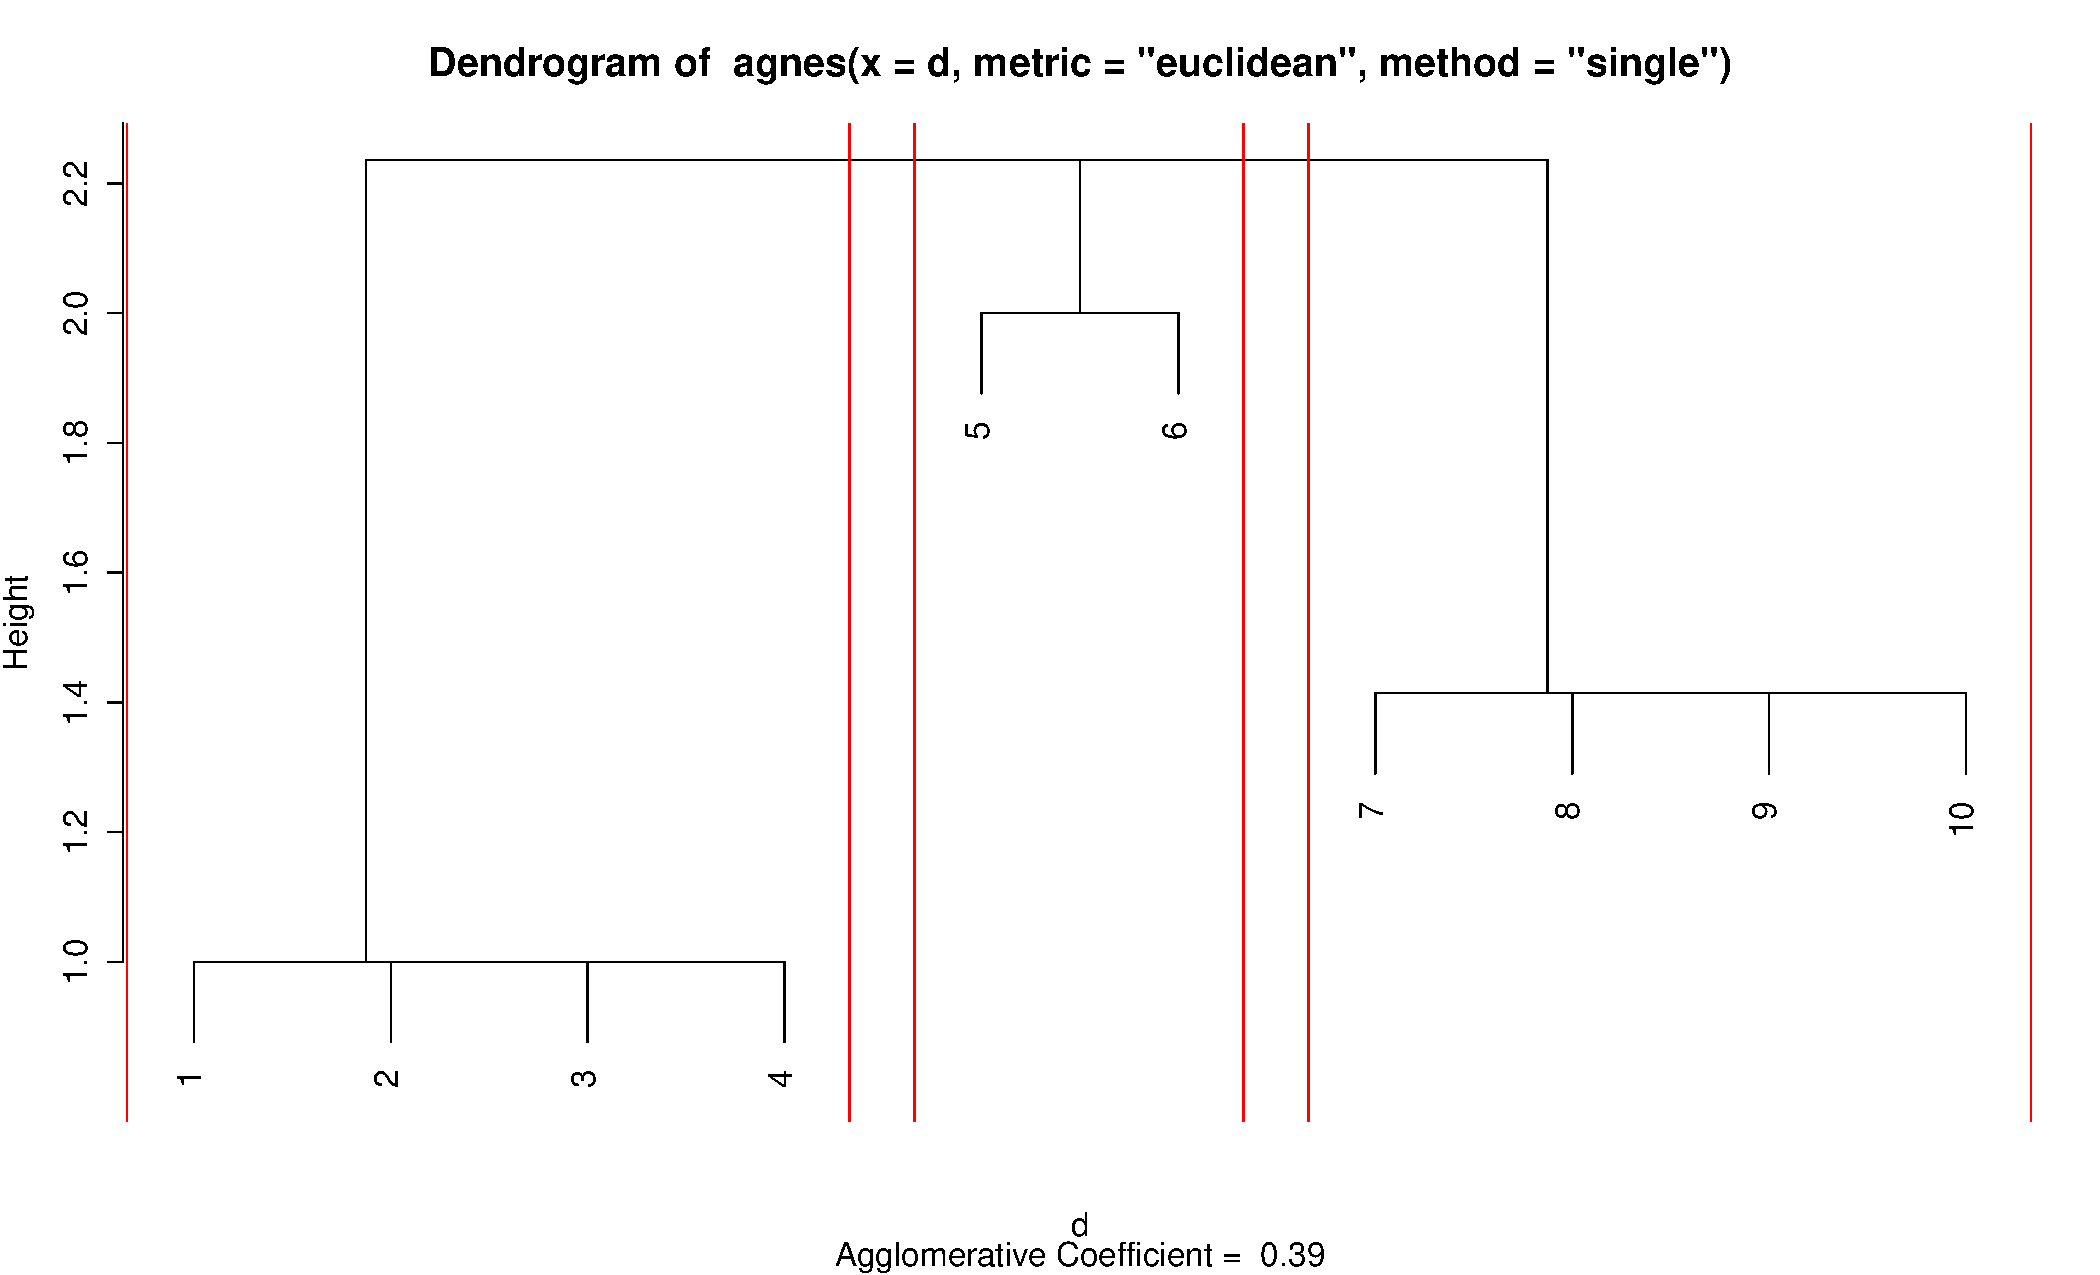
\includegraphics[scale=.35]{images/single-link.pdf}
\end{center}
\end{figure}

\newpage
\subsubsection{Complete Linkage Method}
For this method \textbf{R} produced the following result:

\begin{verbatim}
Call:	 agnes(x = d, metric = "euclidean", method = "complete") 
Agglomerative coefficient:  0.8552376 
Order of objects:
 [1]  1  2  3  4  5  6  7  8  9 10
Height (summary):
   Min. 1st Qu.  Median    Mean 3rd Qu.    Max. 
  1.000   1.414   2.000   2.961   3.000   9.434 

Available components:
[1] "order"  "height" "ac"     "merge"  "diss"   "call"   "method"
[8] "data"
\end{verbatim}

\begin{figure}
\caption{Complete Linkage Graph K=3}
\label{fig:complete}
\begin{center}
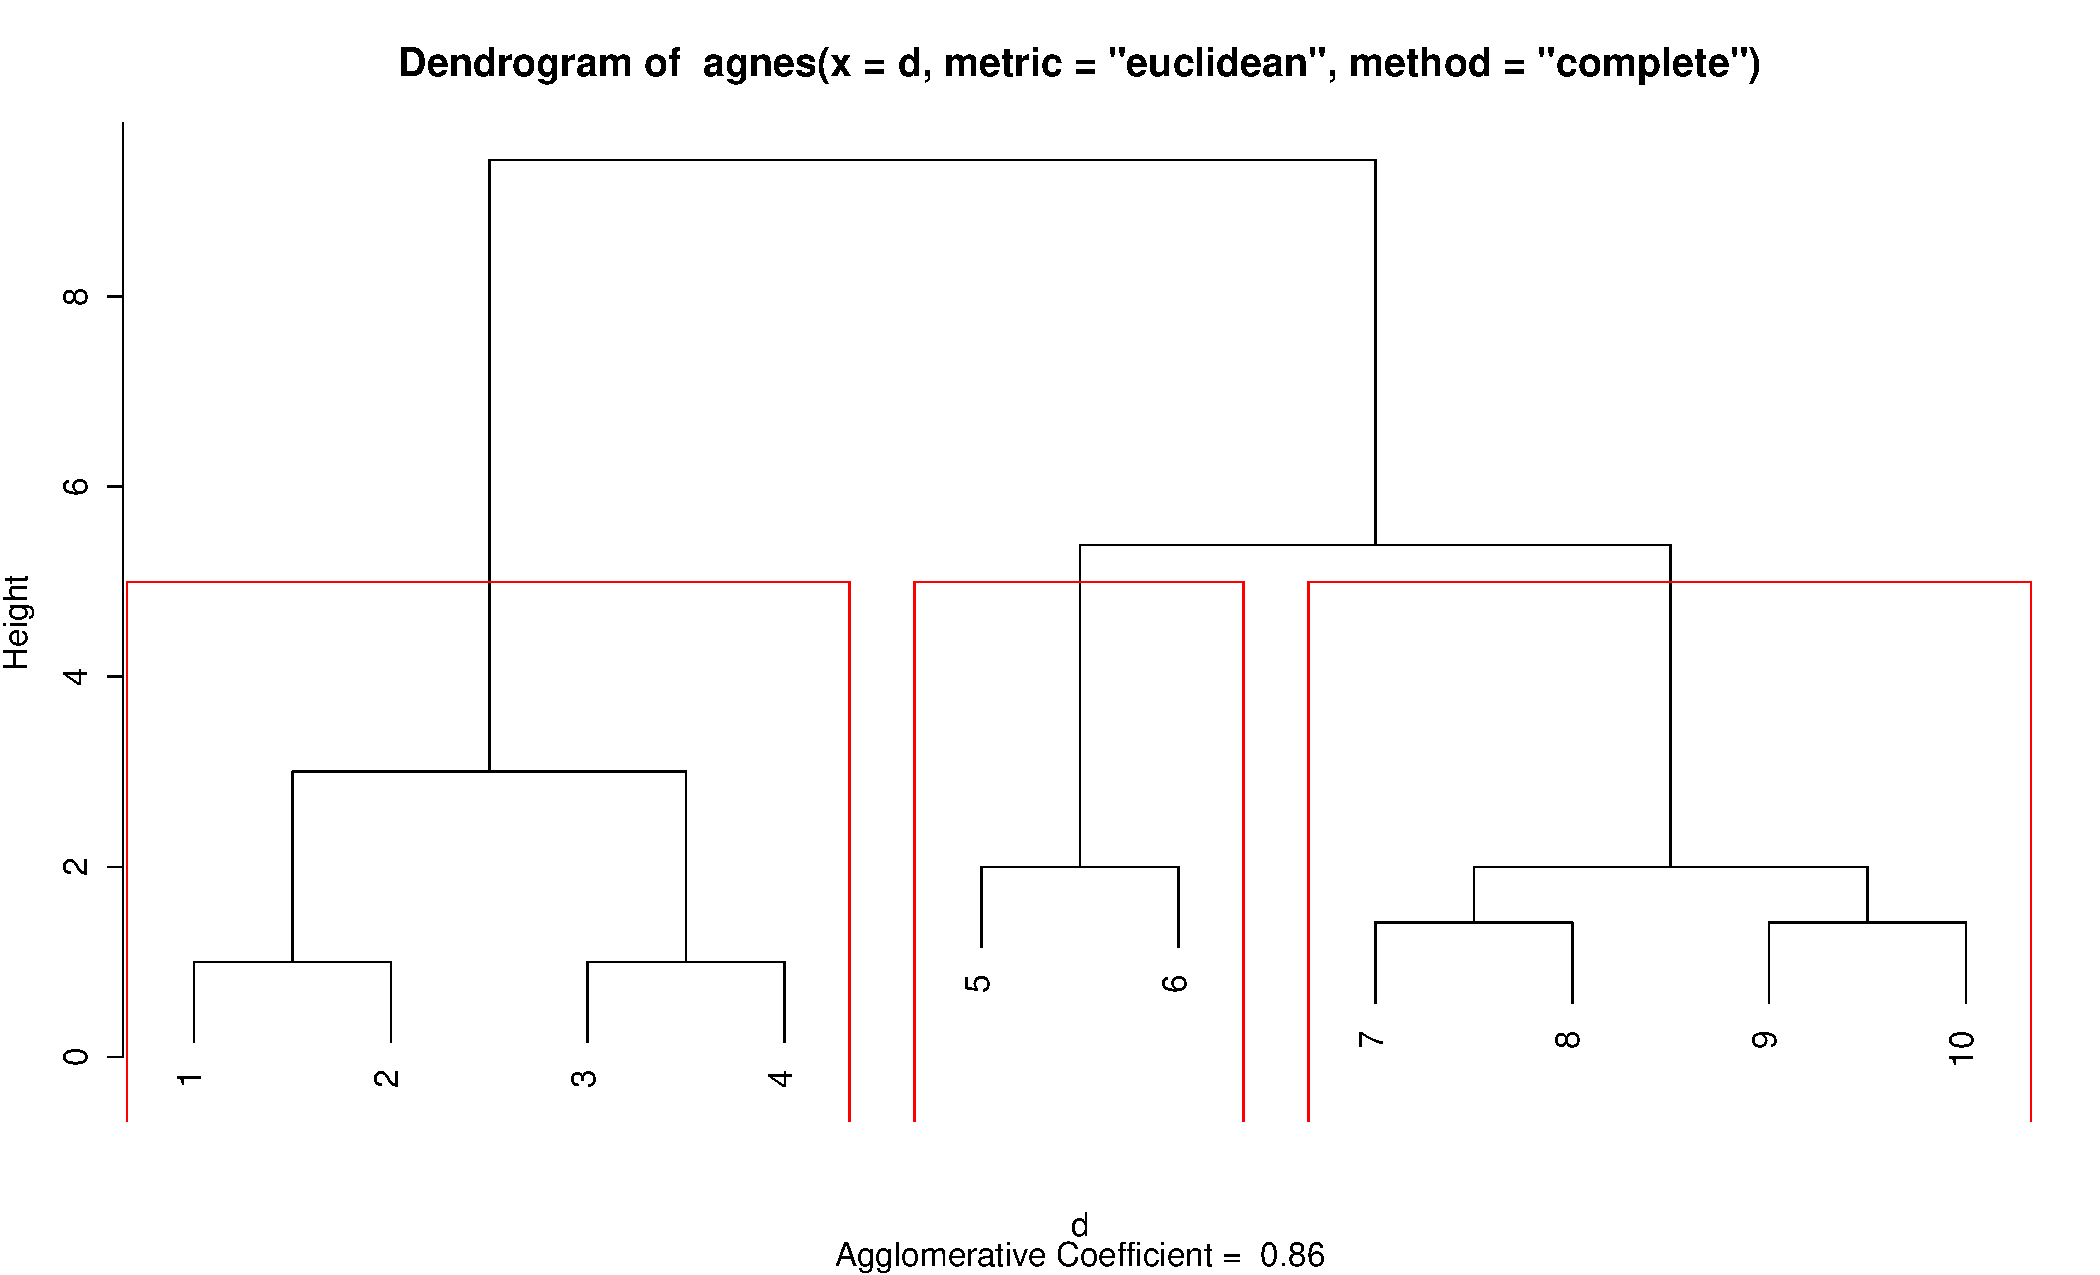
\includegraphics[scale=.35]{images/complete-linkage.pdf}
\end{center}
\end{figure}

\newpage
\subsubsection{Average Linkage}
For this method \textbf{R} produced the following result:

\begin{verbatim}
Call:	 agnes(x = d, metric = "euclidean", method = "average") 
Agglomerative coefficient:  0.7863225 
Order of objects:
 [1]  1  2  3  4  5  6  7  8  9 10
Height (summary):
   Min. 1st Qu.  Median    Mean 3rd Qu.    Max. 
  1.000   1.414   1.707   2.295   2.000   6.391 

Available components:
[1] "order"  "height" "ac"     "merge"  "diss"   "call"   "method"
[8] "data"
\end{verbatim}

\begin{figure}
\caption{Average Linkage Graph K=3}
\label{fig:average}
\begin{center}
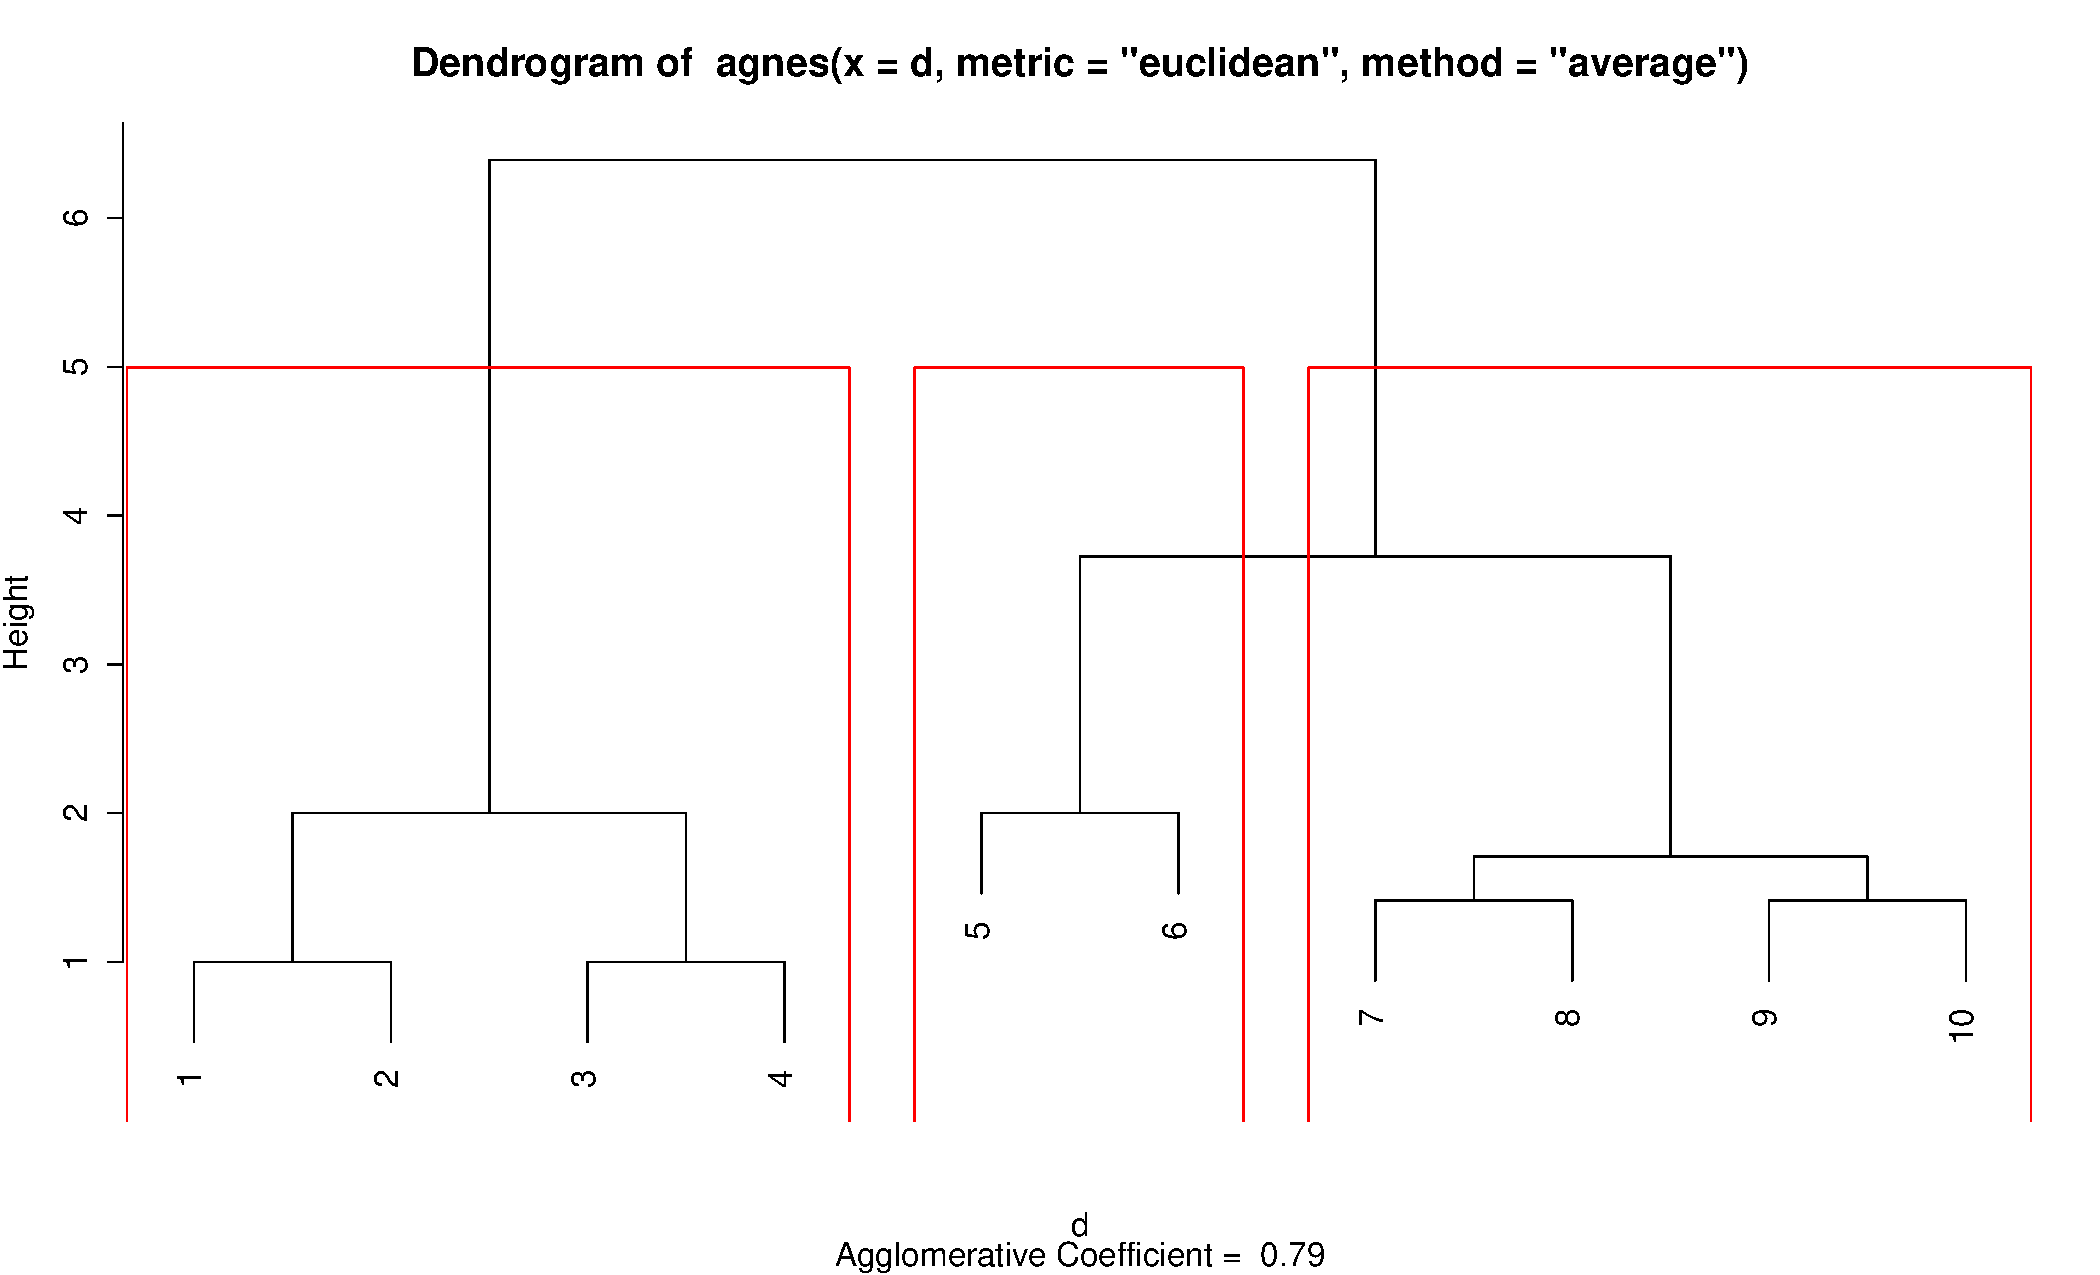
\includegraphics[scale=.35]{images/average.pdf}
\end{center}
\end{figure}

\newpage
\subsubsection{Average Group Linkage}
For this method \textbf{R} produced the following result:

\begin{verbatim}
Call:	 agnes(x = d, metric = "euclidean", method = "gaverage") 
Agglomerative coefficient:  0.8468464 
Order of objects:
 [1]  1  2  3  4  5  6  7  8  9 10
Height (summary):
   Min. 1st Qu.  Median    Mean 3rd Qu.    Max. 
  1.000   1.414   1.769   2.680   2.210   8.917 

Available components:
[1] "order"  "height" "ac"     "merge"  "diss"   "call"   "method"
\end{verbatim}

\begin{figure}
\caption{Average Group Linkage Graph K=3}
\label{fig:average-group}
\begin{center}
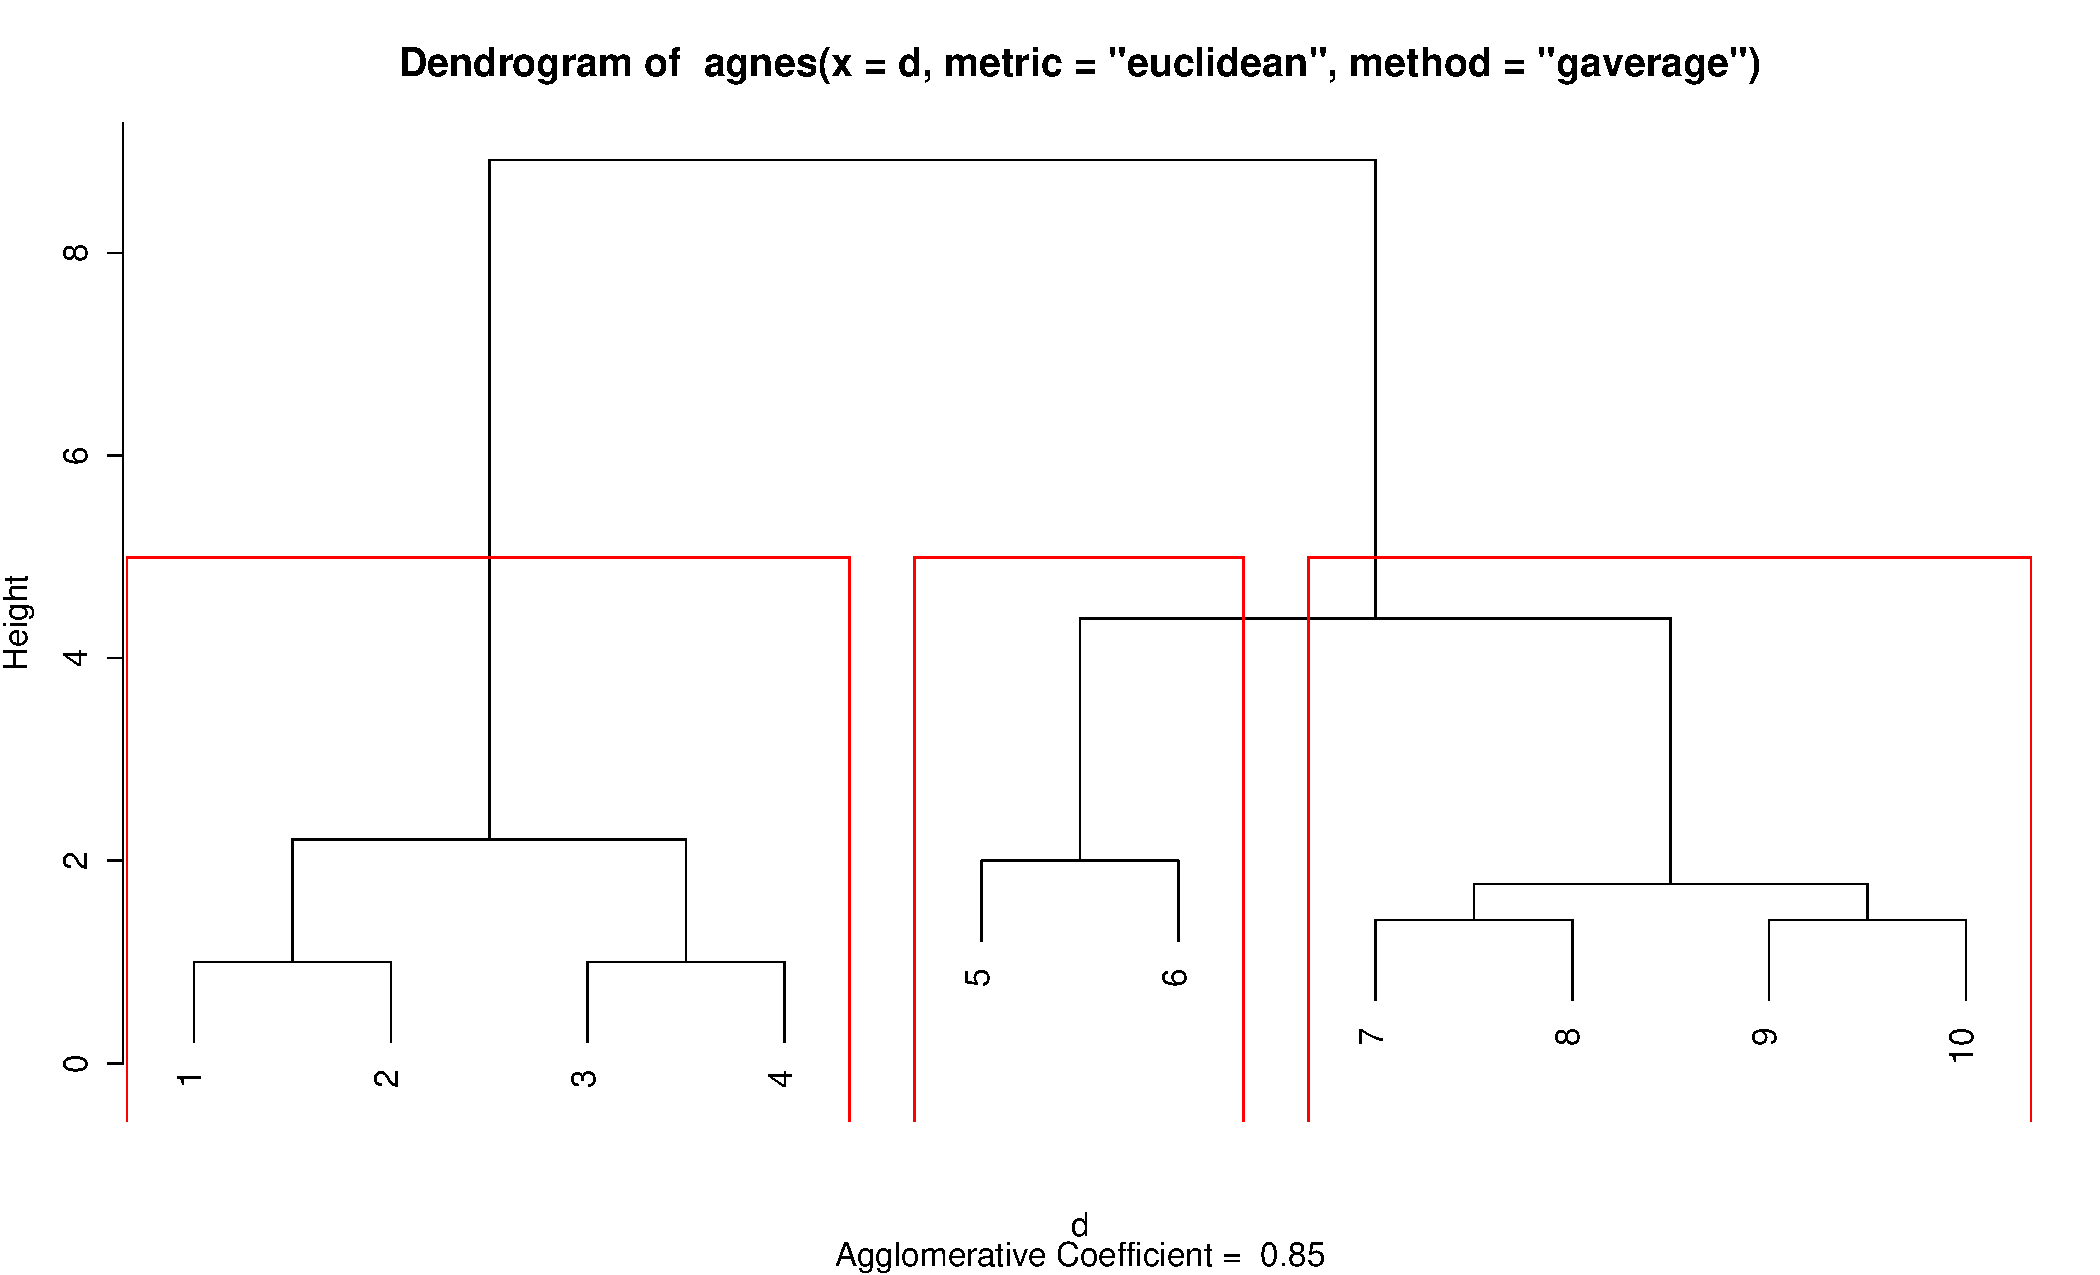
\includegraphics[scale=.35]{images/group-average.pdf}
\end{center}
\end{figure}

\newpage
\subsubsection{Ward’s Method}
For this method \textbf{R} produced the following result:

\begin{verbatim}
Call:	 agnes(x = d, metric = "euclidean", method = "ward") 
Agglomerative coefficient:  0.9006435 
Order of objects:
 [1]  1  2  3  4  5  6  7  8  9 10
Height (summary):
   Min. 1st Qu.  Median    Mean 3rd Qu.    Max. 
  1.000   1.414   2.000   3.477   2.828  13.750 

Available components:
[1] "order"  "height" "ac"     "merge"  "diss"   "call"   "method"
[8] "data"
\end{verbatim}

\begin{figure}
\caption{Ward Graph K=3}
\label{fig:ward}
\begin{center}
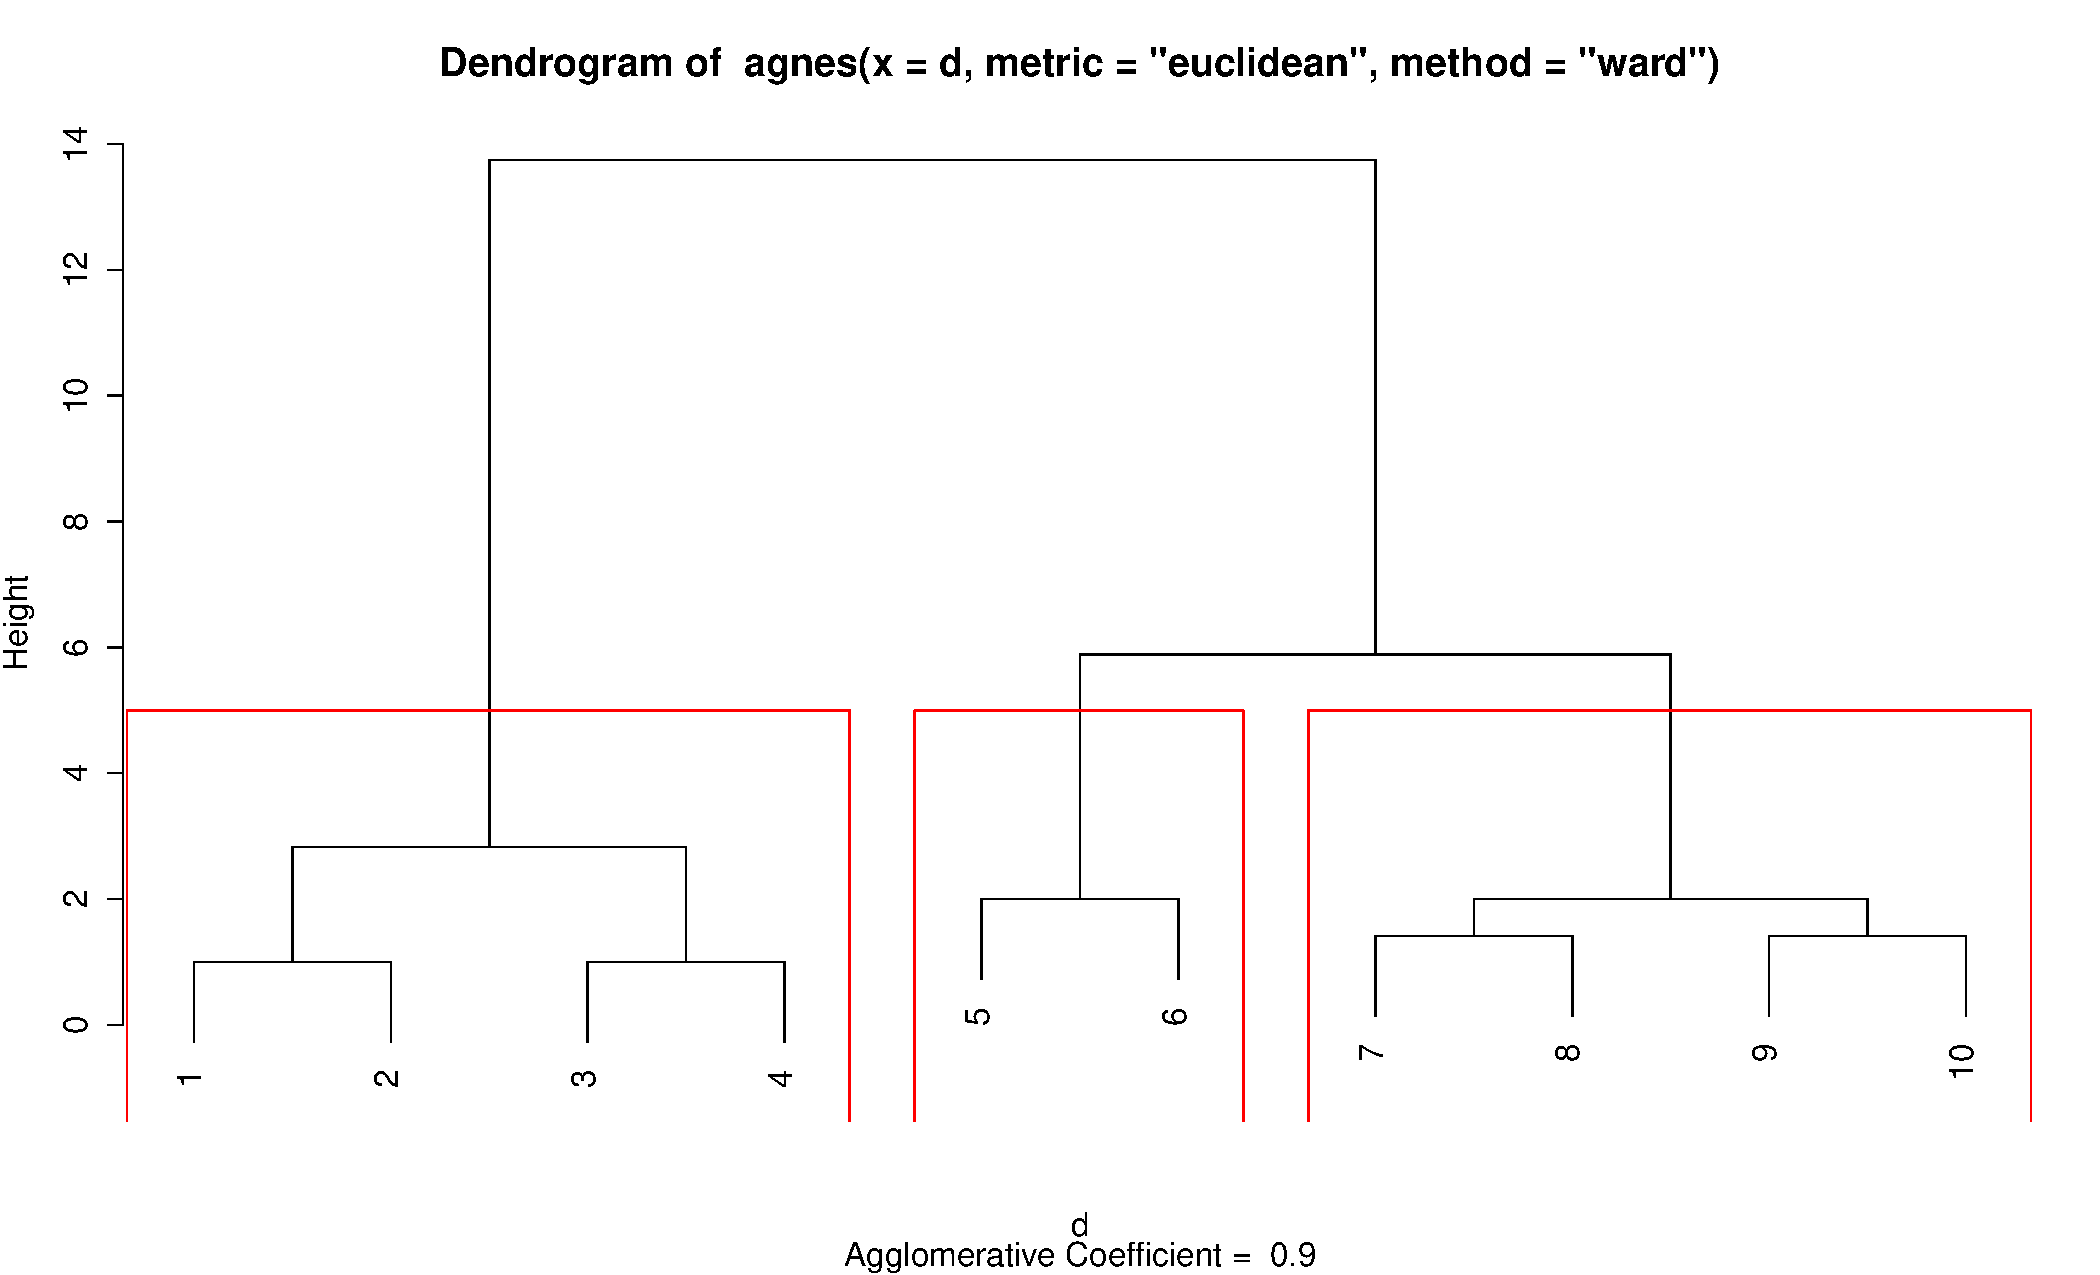
\includegraphics[scale=.35]{images/ward.pdf}
\end{center}
\end{figure}

\subsubsection{Comparison of All Agglomerative Methods}
All five methods resulted in similar clusters of two-dimensional set instances with a $k=3$. However, they differ in the \textit{agglomerative coefficient} which indicates the number of observations required to cluster the set. \\

The \textit{group average linkage} and \textit{complete linkage} have similar agglomerative coefficient, \textbf{0.845} and \textbf{0.855} respectively. Looking at their graphs, they appear to be very similar.\\

The \textit{Single Linkage} has the smallest agglomerative coefficient \textit{0.39}.

\end{homeworkProblem}

%----------------------------------------------------------------------------------------
%	Problem 5
%----------------------------------------------------------------------------------------
\newpage
\begin{homeworkProblem}[Exercise 9.10]% Custom section title
\vspace*{10pt} % Question
Nearest neighbor clusters are not symmetric, in the sense that if instance A
is one of instance B’s nearest neighbors, the reverse is not necessarily true. Explain how this can happen with a diagram.\\

Figure \ref{fig:asymmetric} is an instance which shows nearest neighbor clusters are not symmetric. For example, the figure shows that if we were going to cluster the set with $k=2$, the nearest neighbor for $A$ would be $B$, however for $B$ the nearest neighbors are $D$ and $C$. Proving that nearest neighbor clusters are not symmetric.


\begin{figure}[h]
\caption{Asymmetric Nature of Nearest Neighbor}
\label{fig:asymmetric}
\begin{center}
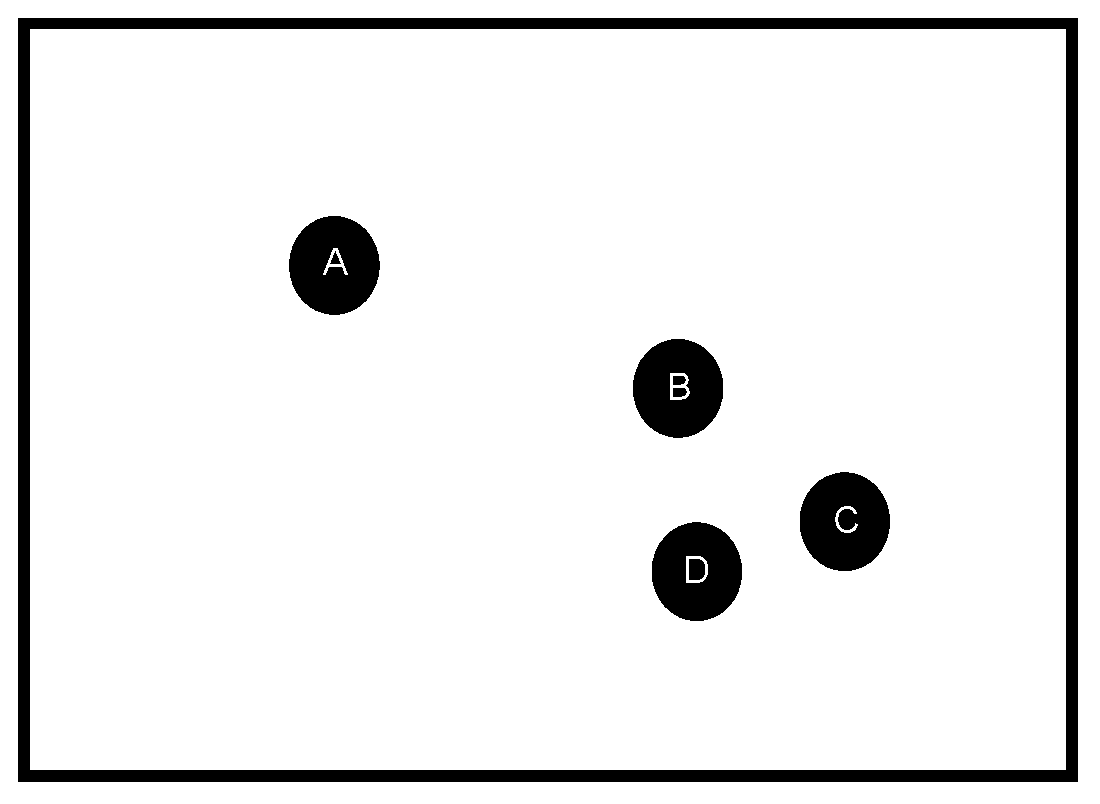
\includegraphics[scale=.30]{images/k-nn.pdf}
\end{center}
\end{figure}
\end{homeworkProblem}
%----------------------------------------------------------------------------------------
%	Bibliography
%----------------------------------------------------------------------------------------
\newpage
\bibliography{bibliography}
\bibliographystyle{siam}
%\begin{thebibliography}{9}
%\bibitem{Lutz} 
%Lutz, Mark (2013). List and Dictionaries. \textit{Learning Python} (5th ed.). (pp. %262-263). Sebastopol, CA: O'Reilly Media.
%
%\bibitem{ci}
%Segarn, Toby. Programming Collective Intelligence. \textit{Building Smart Web 2.0 Application}. (pp 29-53). Sebastopol, CA: O'Reilly Media.

%\bibitem{sitemaps}
%Sitemaps Schema. (n.d.) Retrieved September 21, 2016, from \url{http://www.sitemaps.org/schemas/sitemap/0.9}

%\end{thebibliography}
\end{document}